\chapter{Veto Efficiency Studies}\label{chap:VetoEfficiency}
A WIMP scatter should only deposit a small amount of energy (few~keV) within the LXe volume of the experiment without any simultaneous energy deposit in the surrounding materials. Neutrons produced through radioactive decays within detector materials would mimic a WIMP interaction when they scatter off Xe atoms. 

%A WIMP scatter would deposit a few keV in the central volume of the LXe TPC, with no simultaneous energy deposit in surrounding materials. Neutrons caused by radioactivity, which can fake WIMP interactions when they scatter elastically, are likely to interact again either within the TPC or nearby, and so it is broadly desirable to replace as much of the neighboring material as possible with additional radiation detectors. It also helps to minimize intervening material between the active LXe in the TPC and any such ancillary detectors, namely by decreasing the thickness of the field-cage and of the cryostat vessels. Active material surrounding the central LXe volume also permits assessment of the local radioactivity environment, and thus to infer additional information on the backgrounds in the WIMP search region. A persuasive WIMP discovery will require excellent understanding of all background sources, which is best done through the characterization of those sources in situ.
\section{Simulation Matching}\label{sec:simulation_improvements}
\subsection{Tuning OD}
\subsubsection{Geometry Edits}\label{sec:GeometryEdits}
Prior to WS2024 result, there were a number of major differences between simulations and data in the Outer Detector. 
As such, an effort was made to correct this. 
The changes made were;
\begin{enumerate}
    \item A gap was added between the acrylic tanks to account for the gap seen during installation.
    \item Water was added to the foam volume which is between the OCV and acrylic tanks; each 
    \item The acrylic tanks were moved further away from the OCV; this matches what adding the gaps was supposed to solve.
\end{enumerate}

The percentage of water in the foam, and the outward movement of the acrylic tanks were looped over.
The water percentage of the foam was increased in 1\% steps, and the acrylic tanks were moved by 10mm steps.
The 'best' value was found to be 30mm and 6\%.
Additional details on the discrepancies between simulations and data are shown in the subsequent subsections.

\begin{figure}
    \centering
    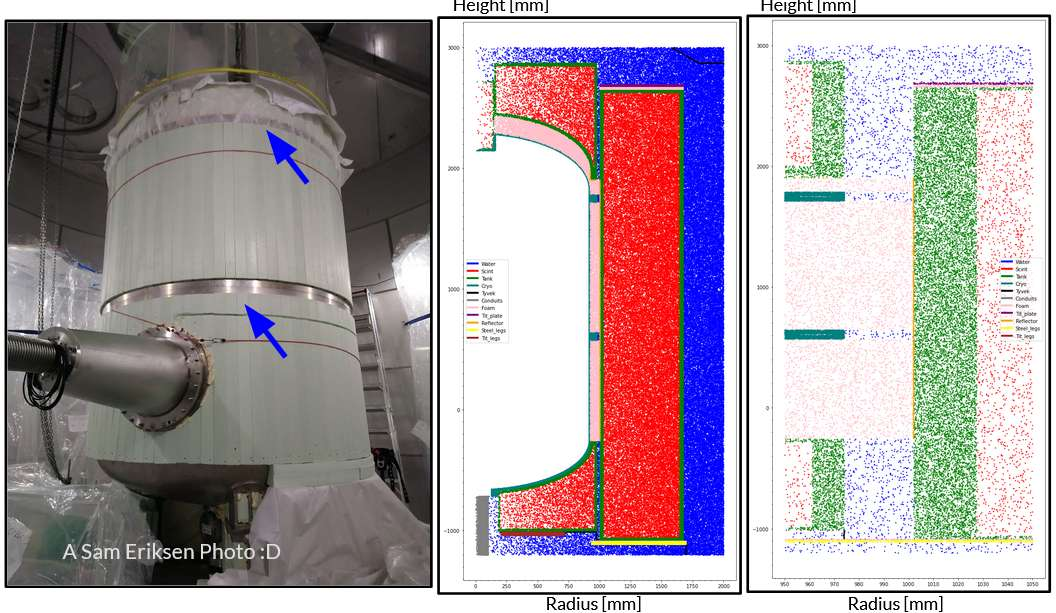
\includegraphics[width=0.8\textwidth]{figures/VetoEfficiency/Final_OD_geometry.png}
    \caption{Geometry in the simulation used for SR3.}
    \label{fig:od_geometry_for_sr3}
\end{figure}

\subsubsection{Capture Time}
Following the geometry changes discussed above, the neutron capture timing using AmLi was studied. Prior to the geometry changes, there was a distinct discrepancy between data and simulation when considering neutron capture timing following single scatters within the TPC. Initial skims of both data and simulation were made using ALPACA, selecting all events which were classified as single scatters by LZAP. OD pulse information was also skimmed considering 100~keV (24~phd), 200~keV (49~phd) and 1~MeV (251~phd) OD thresholds.
The simulation was modified in two different ways, moving the SATs out radially and adding water to the foam. All possible configurations were visually examined to determine which variation of simulation matched the data. An example of the comparison plot can be seen in \autoref{fig:NC_AmLi_50mm7}, the "baseline simulation" was the initialy configuration of the geometry prior to this study. All plots were examined side by side in a large scale canvas configuration seen in \autoref{fig:NC_Canvas}. It was found that from this study that 30~mm~to~50~mm movement of the SATs alongside 5\%~to~7\% increase in the percentage of water in the foam provides the best agreement between data and simulation at a 200~keV threshold.
\begin{figure}
    \centering
    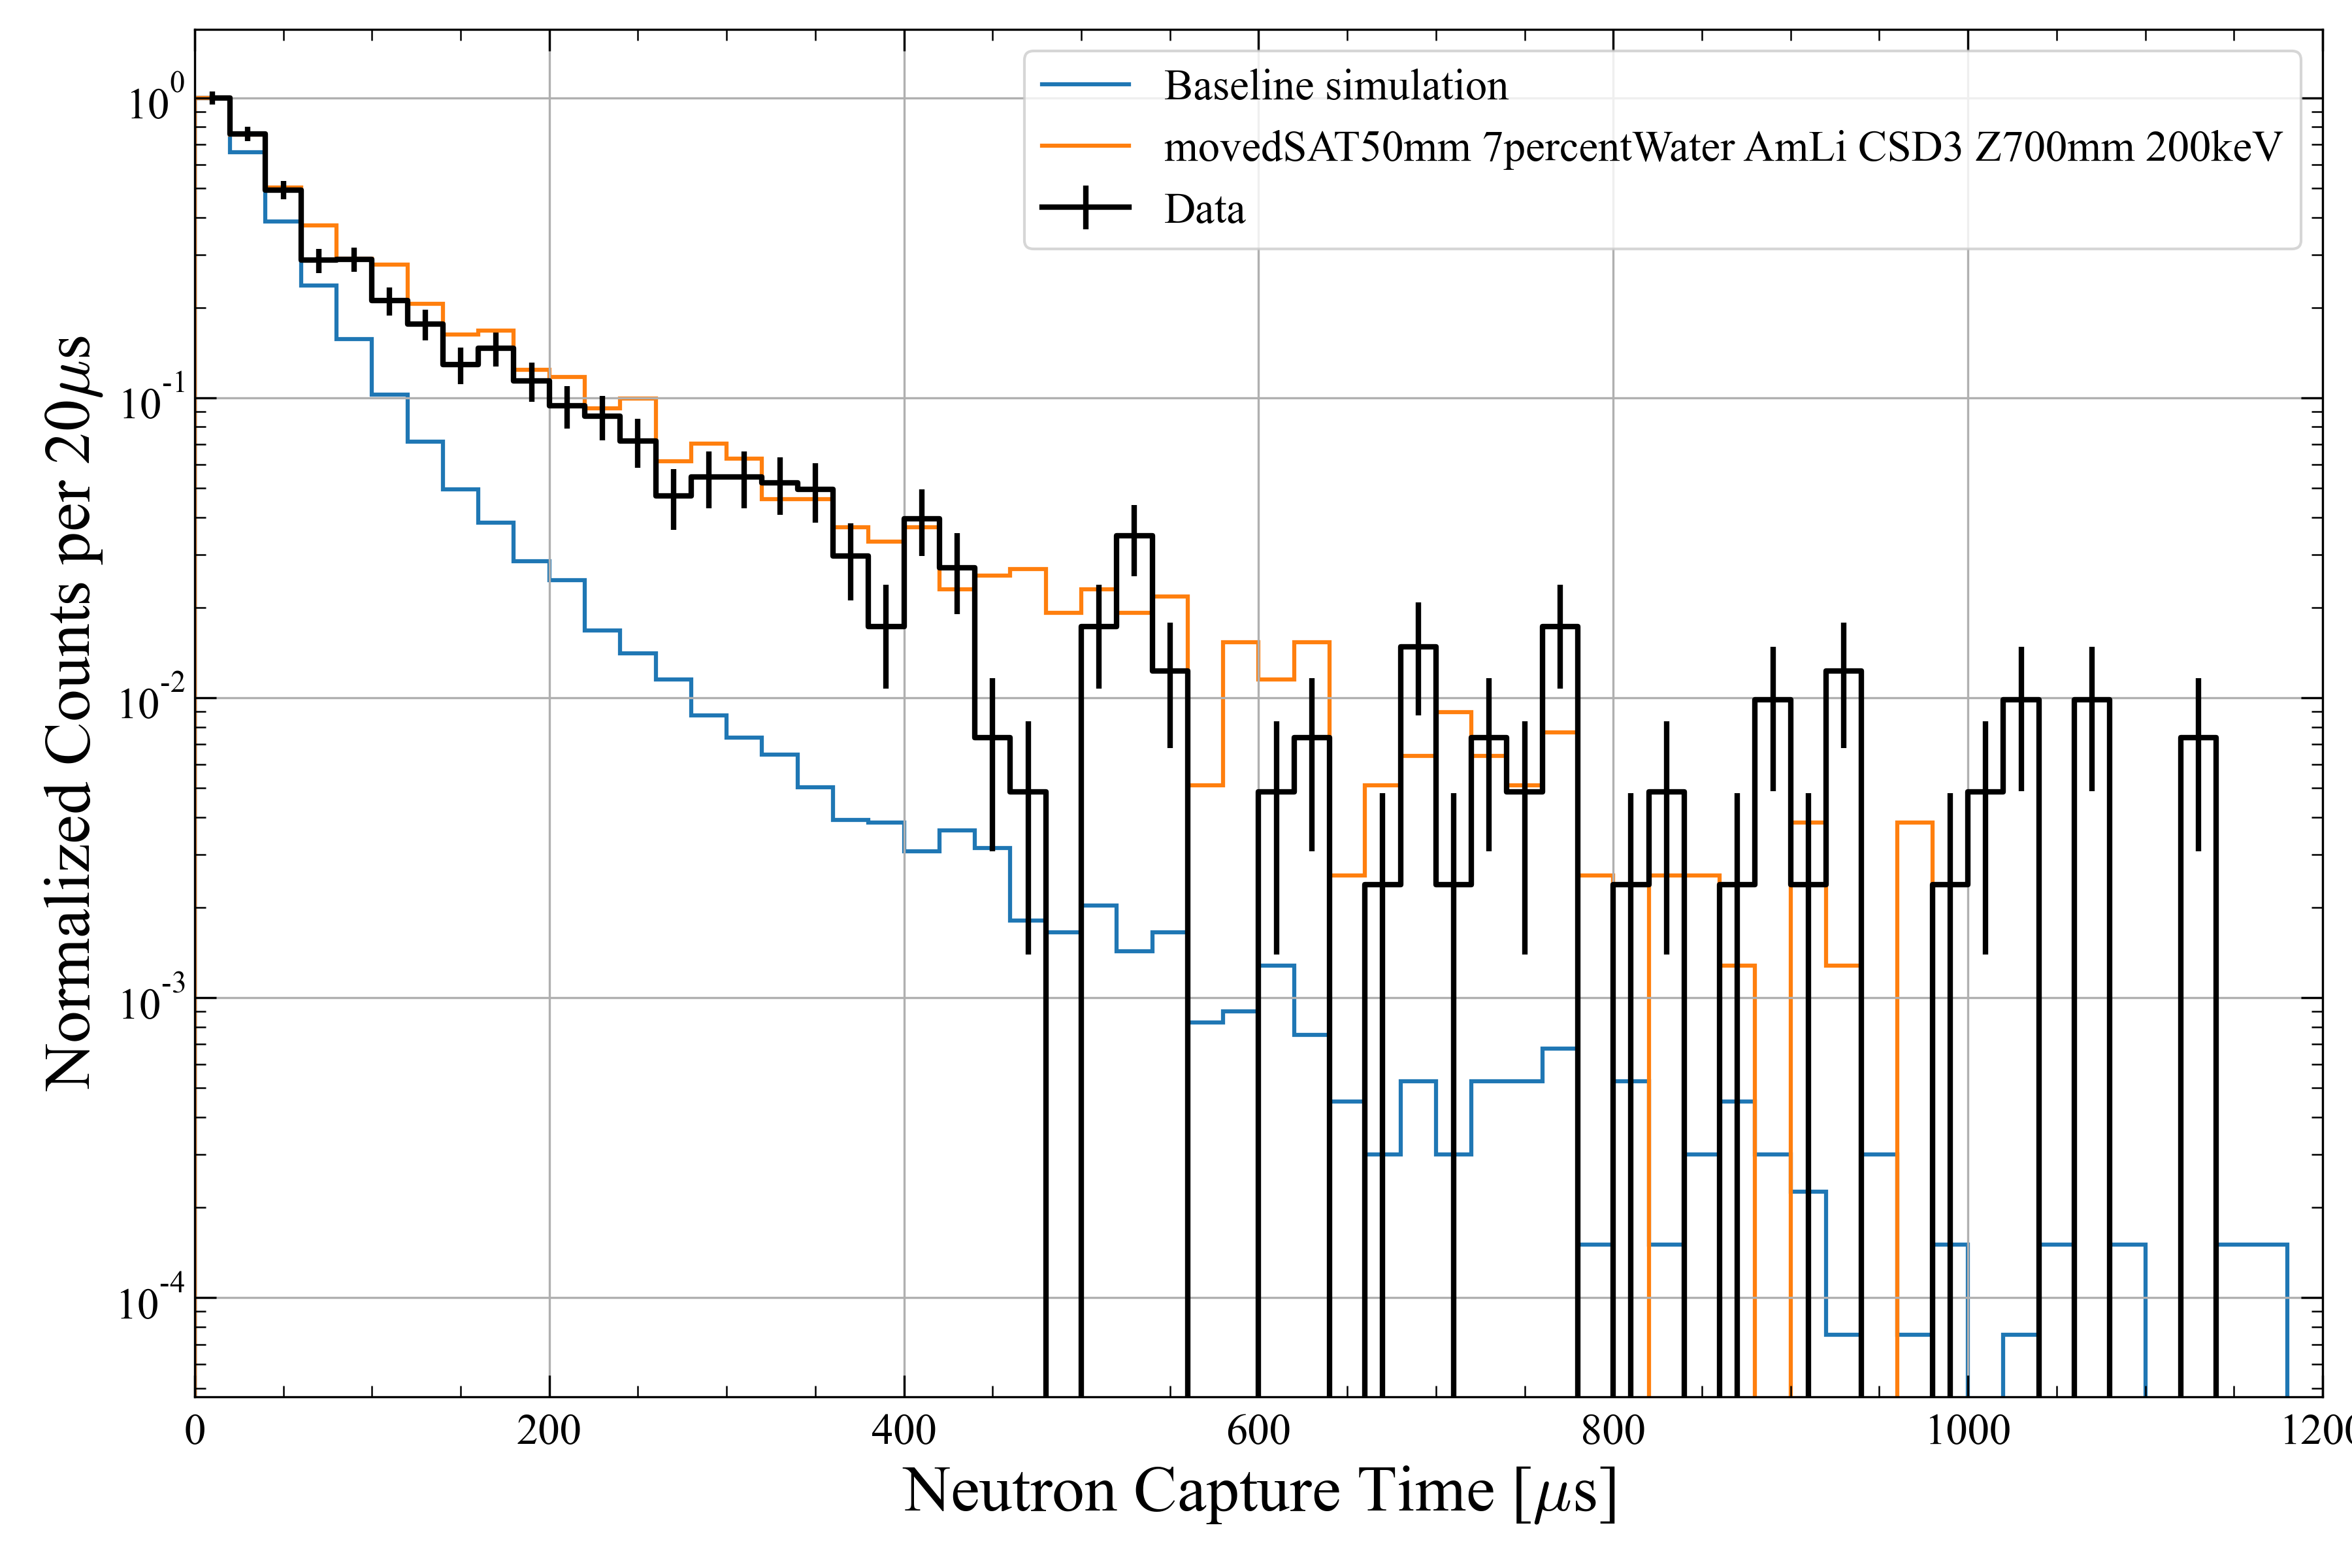
\includegraphics[width=0.8\linewidth]{figures/VetoEfficiency/movedSAT50mm_7percentWater_AmLi_CSD3_Z700mm_200keV.png}
    \caption{An example of the plot used to compare neutron capture timing in data with the baseline simulation and the modified simulation.}
    \label{fig:NC_AmLi_50mm7}
\end{figure}
\begin{figure}
    \centering
    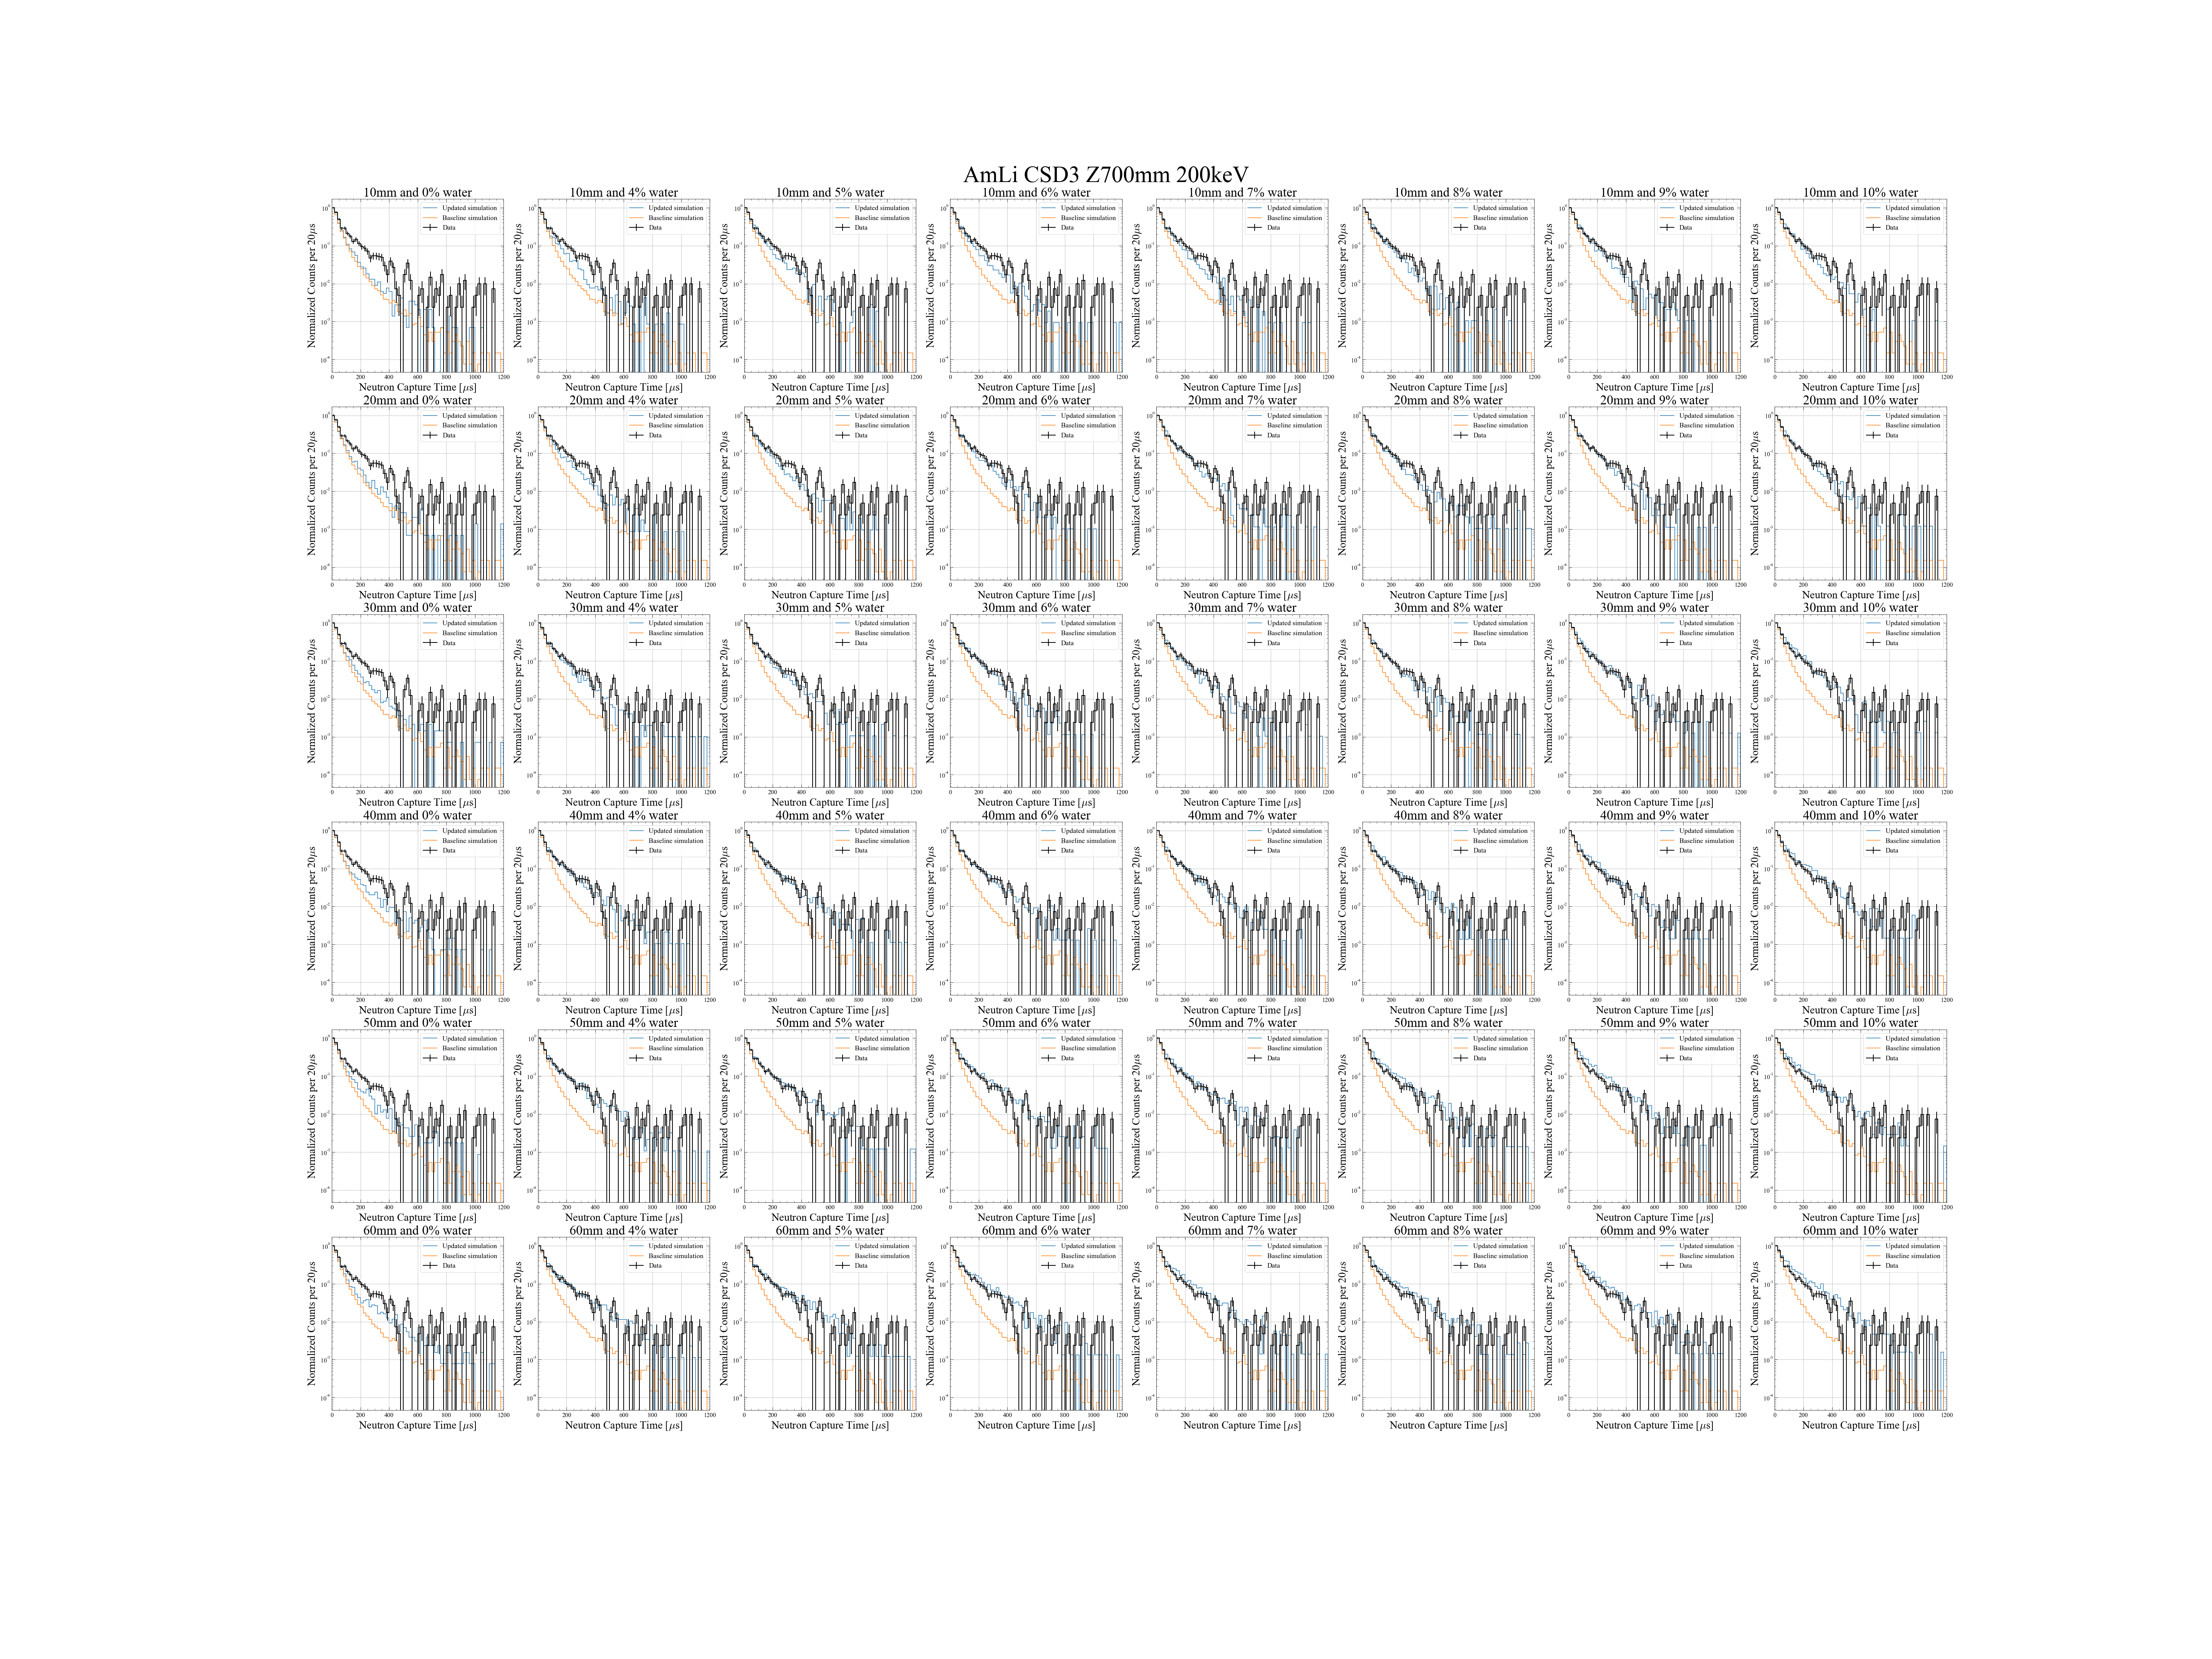
\includegraphics[width=\linewidth]{figures/VetoEfficiency/AmLi_CSD3_Z700mm_200keV.png}
    \caption{Large scale canvas of all possible simulation configurations. Each plot is similar in style to \autoref{fig:NC_AmLi_50mm7}. Here AmLi at 700mm in CSD3 has been shown as an example.}
    \label{fig:NC_Canvas}
\end{figure}

\section{Veto Selection Optimisation}
In this section, details on how the Skin and OD cuts used in SR3 were created are defined. The Skin and OD veto cuts used in SR3 were based on those developed for SR1, described in \cite{LZCollaboration:2024lux}.
This boils down to four cuts;
\begin{itemize}
    \item Skin-prompt: For tagging $\gamma$-rays in the Skin detector,
    \item OD-prompt: For tagging $\gamma$-rays and neutron proton recoils in the OD detector,
    \item Skin-delayed: For tagging $\gamma$-rays from post-neutron capture de-excitation,
    \item OD-delayed: For tagging $\gamma$-rays from post-neutron capture de-excitation.
\end{itemize}

Using SR1 (and pre-SR2) as a baseline, three studies were performed to adapt these cuts for SR3;
\begin{enumerate}
    \item Determine the detector stability, to establish if the energy scale for the detectors has changed; using this the SR1 cuts can simply be scaled for SR3, and asks as a starting point.
    \item Implement a position correction to the OD.
    \item Perform cut optimisation based on the above studies.
\end{enumerate}

The cuts used for the vetoes were selected at the same time as AmLi neutron tagging efficiency calculation, and were set to maximise the tagging efficiency whilst reducing deadtime\footnote{in future, a PLR study should be done to determine at what point this is optimaised}.
As such, this section should be considered simultaneously with \autoref{sec:AmLi_Efficiency}

On a skim of the AmLi calibrations which pass the SR3 core-cuts described in \autoref{tab:amli_efficiency_cuts}, the efficiency (described in \autoref{eq:neutron_tagging_efficiency}) was calculated with the pulse area, and coincidence thresholds of the Skin and OD varying in integer steps.
This then produces a heatmap of the coincidence vs. threshold vs. efficiency of each cut, examples of these are shown in \autoref{fig:od_prompt_veto_heatmap}-\ref{fig:skin_delayed_veto_heatmap}. 
For the delayed cuts, the veto time window was also varied, and heatmaps of threshold vs. time window vs. efficiency were produced for a fixed coincidence. Heatmaps with dead time rather than efficiency were also produced. The dead time is discussed in greater detail in the next section. 

The windows for the prompt cuts were selected by looking at the DD and AmLi calibrations (the run numbers and the LZAP version are listed in \autoref{sec:efficiency}) and by measuring the time difference between the TPC single-scatter and OD and Skin pulses.
For Amli, this is shown in \autoref{fig:veto_prompt_windows}.

Compiling the heat maps of efficiency and deadtime for a variety of veto windows, a choice of thresholds were chosen to maximise efficiency whilst minimising dead time.
An example plot we used to determine this is shown in \autoref{fig:veto_cut_optimisation}.
For SR3, we took the approach of trying to maintain the efficiency of SR1 veto of $\sim$~90\%, and to reduce the livetime impact.
From the heatmaps, we determined that we could achieve an efficiency that at least matched the SR1 efficiency, but with a much lower deadtime.
The final cuts are shown in \autoref{fig:sr3_veto_cuts}.

\begin{figure}
     \centering
     \begin{subfigure}[b]{0.48\textwidth}
         \centering
         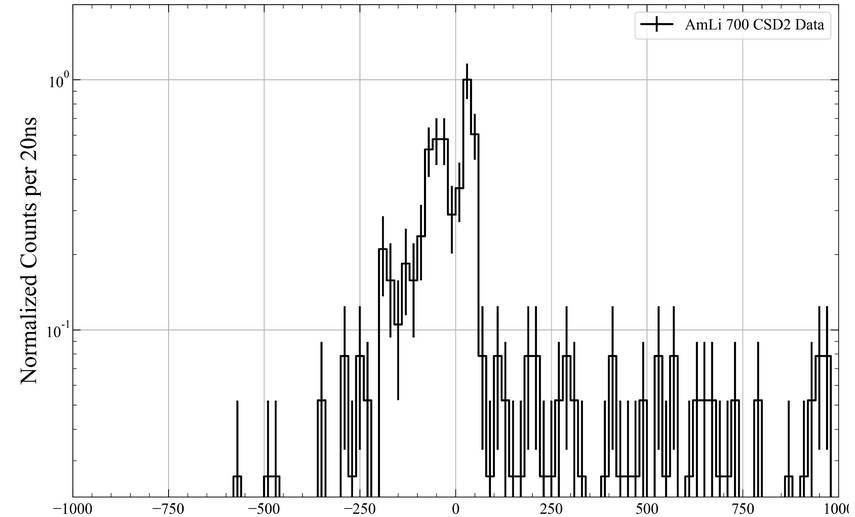
\includegraphics[width=\textwidth]{figures/VetoEfficiency/skin_prompt.png}
         \caption{Time difference (in ns) between TPC single-scatter and Skin pulses.
         To reduce the noise in the plot, a pulse requirement of greater than 2~phd and greater than 2~coincidence has been applied to the Skin pulses}
         \label{fig:skin_prompt_window}
     \end{subfigure}
     \hfill
     \begin{subfigure}[b]{0.48\textwidth}
         \centering
         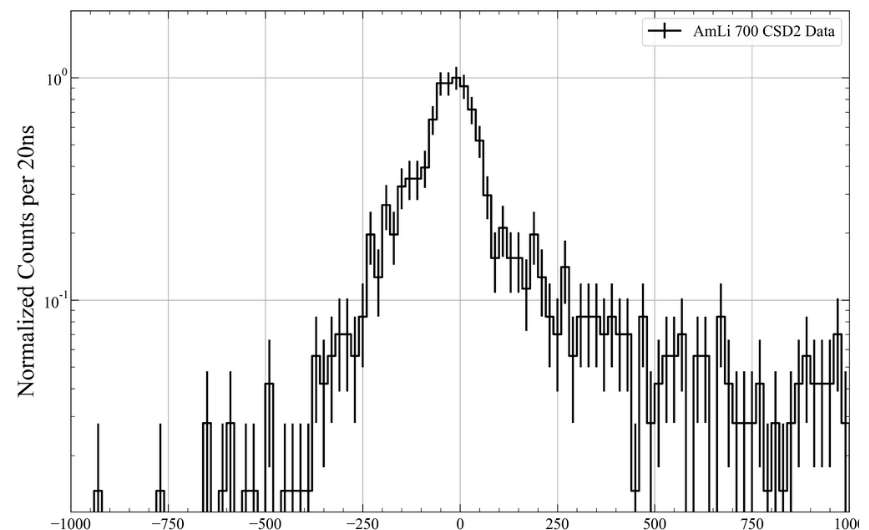
\includegraphics[width=\textwidth]{figures/VetoEfficiency/od_prompt.png}
         \caption{Time difference (in ns) between TPC single-scatter and OD pulses.
         To reduce the noise in the plot, a pulse requirement of greater than 5~phd and greater than 22~coincidence has been applied to the OD pulses}
         \label{fig:od_prompt_window}
     \end{subfigure}
    \caption{Time difference between TPC single-scatter and Veto pulses.
    This is used to determine the prompt veto windows.}
    \label{fig:veto_prompt_windows}
\end{figure}


\begin{sidewaysfigure}
    \centering
    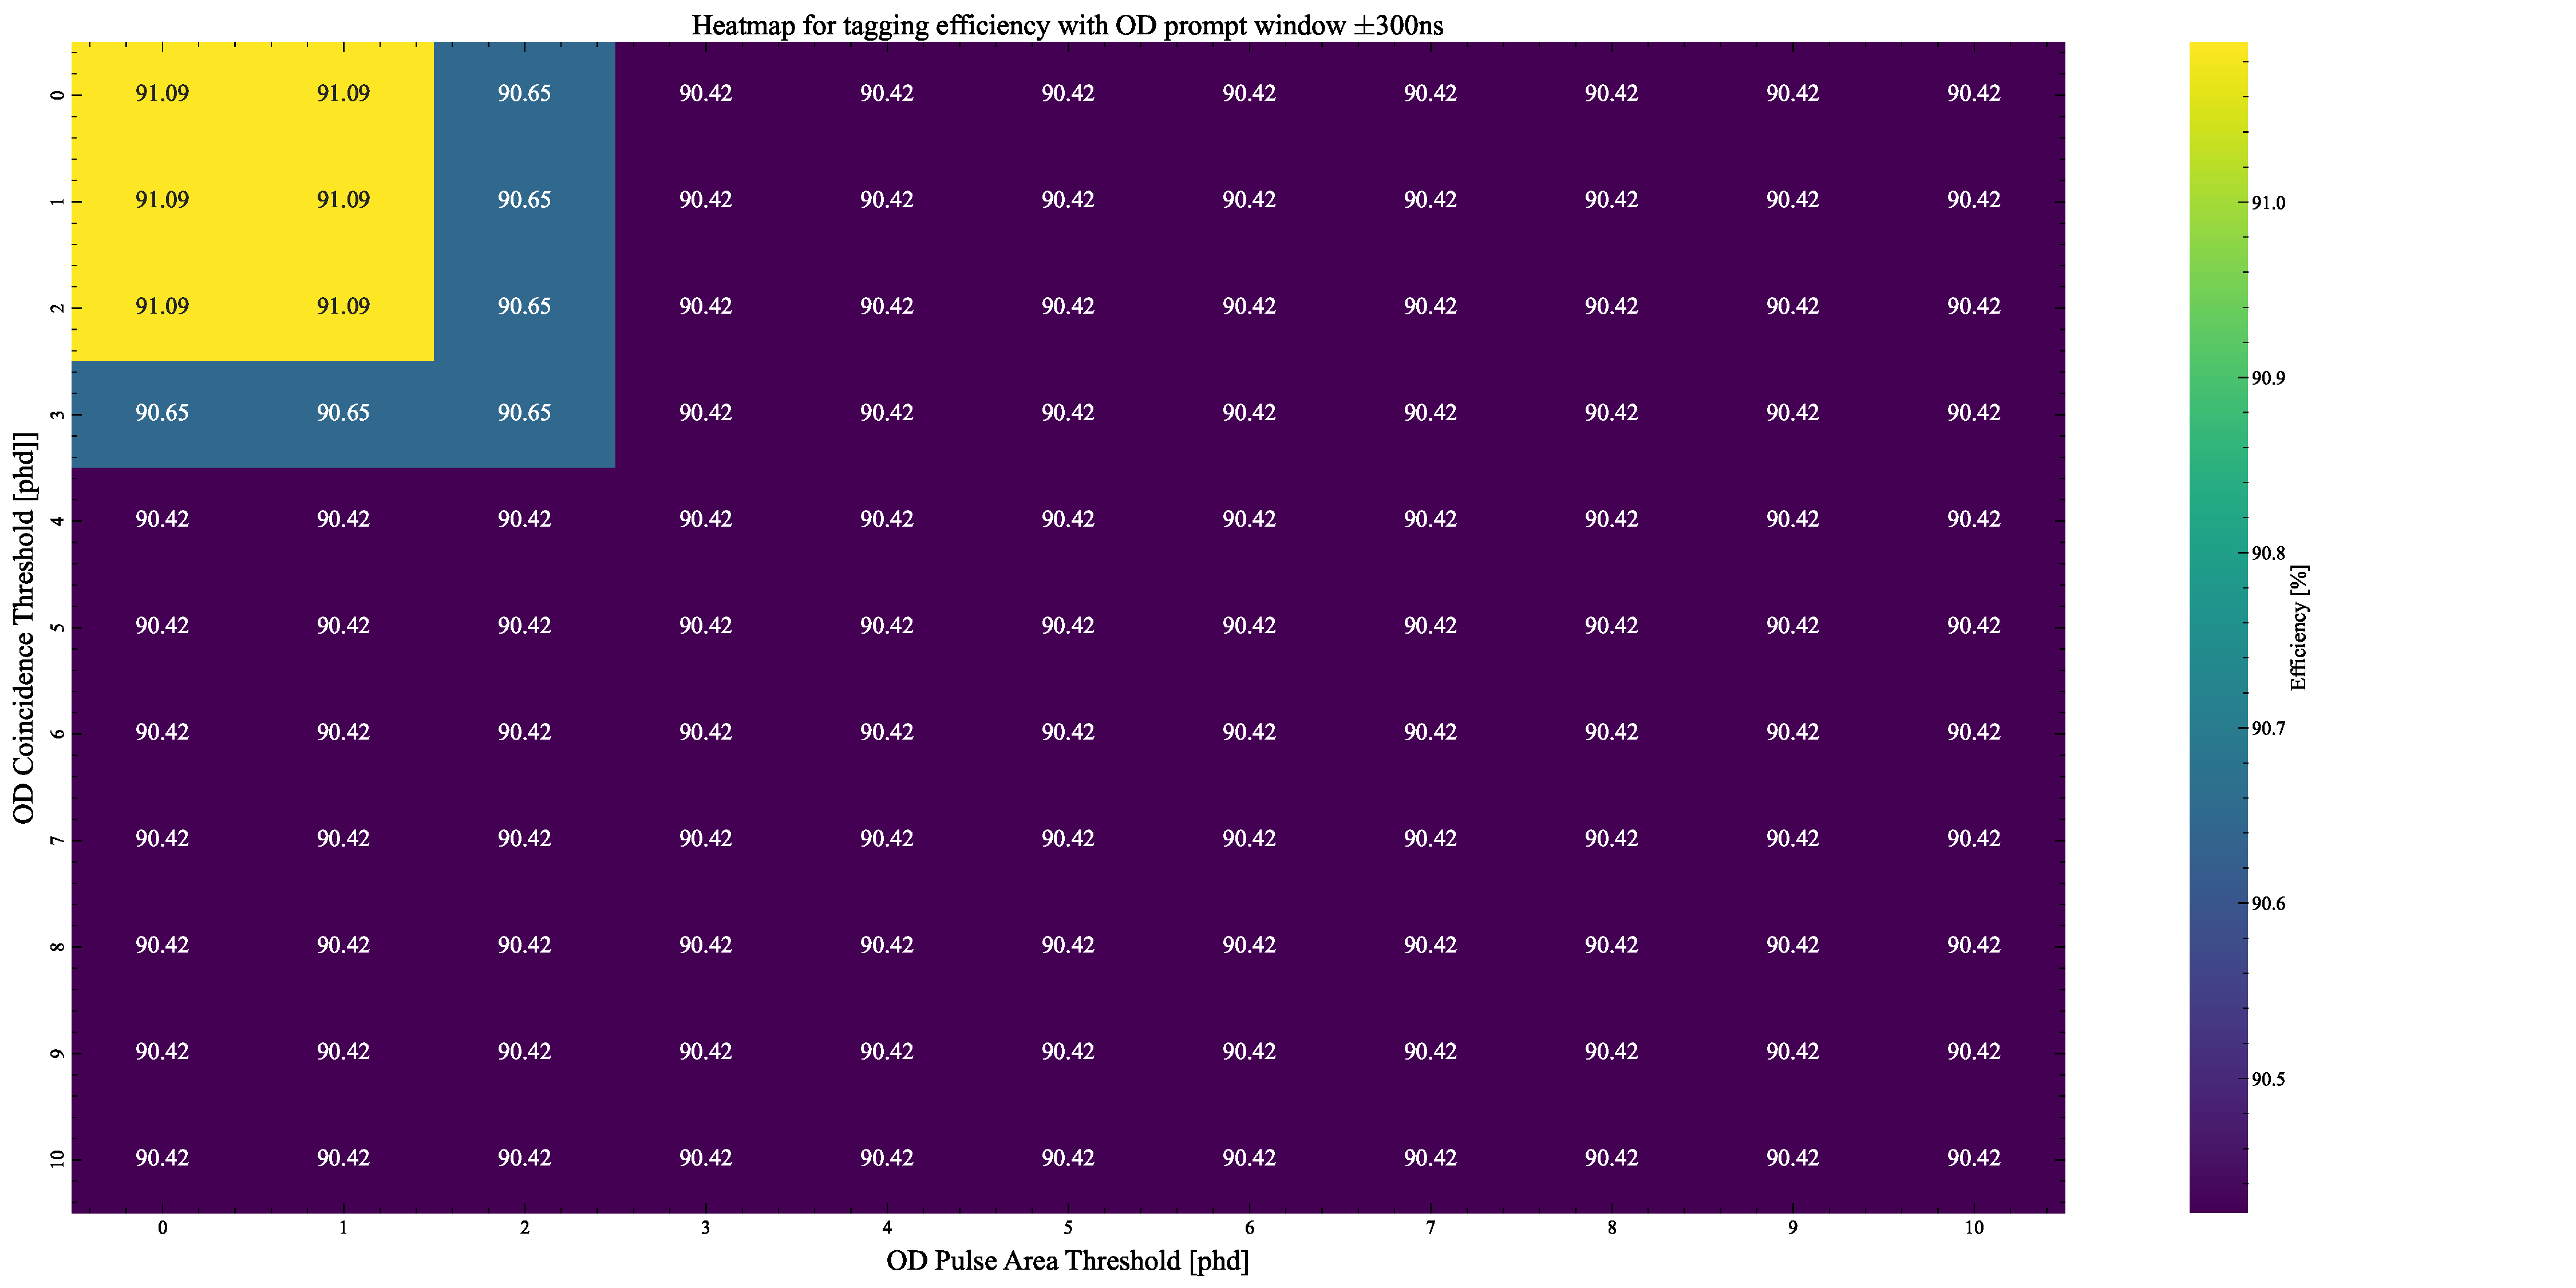
\includegraphics[width=\textwidth]{figures/VetoEfficiency/HeatmapODPACoinScanWindow600.pdf}
    \caption{OD Prompt heatmap. 
    The z-axis shows the efficiency associated with a given pulse requirement.
    The veto time window considered is [-300, 300]ns.
    }
    \label{fig:od_prompt_veto_heatmap}
\end{sidewaysfigure}

\begin{sidewaysfigure}
    \centering
    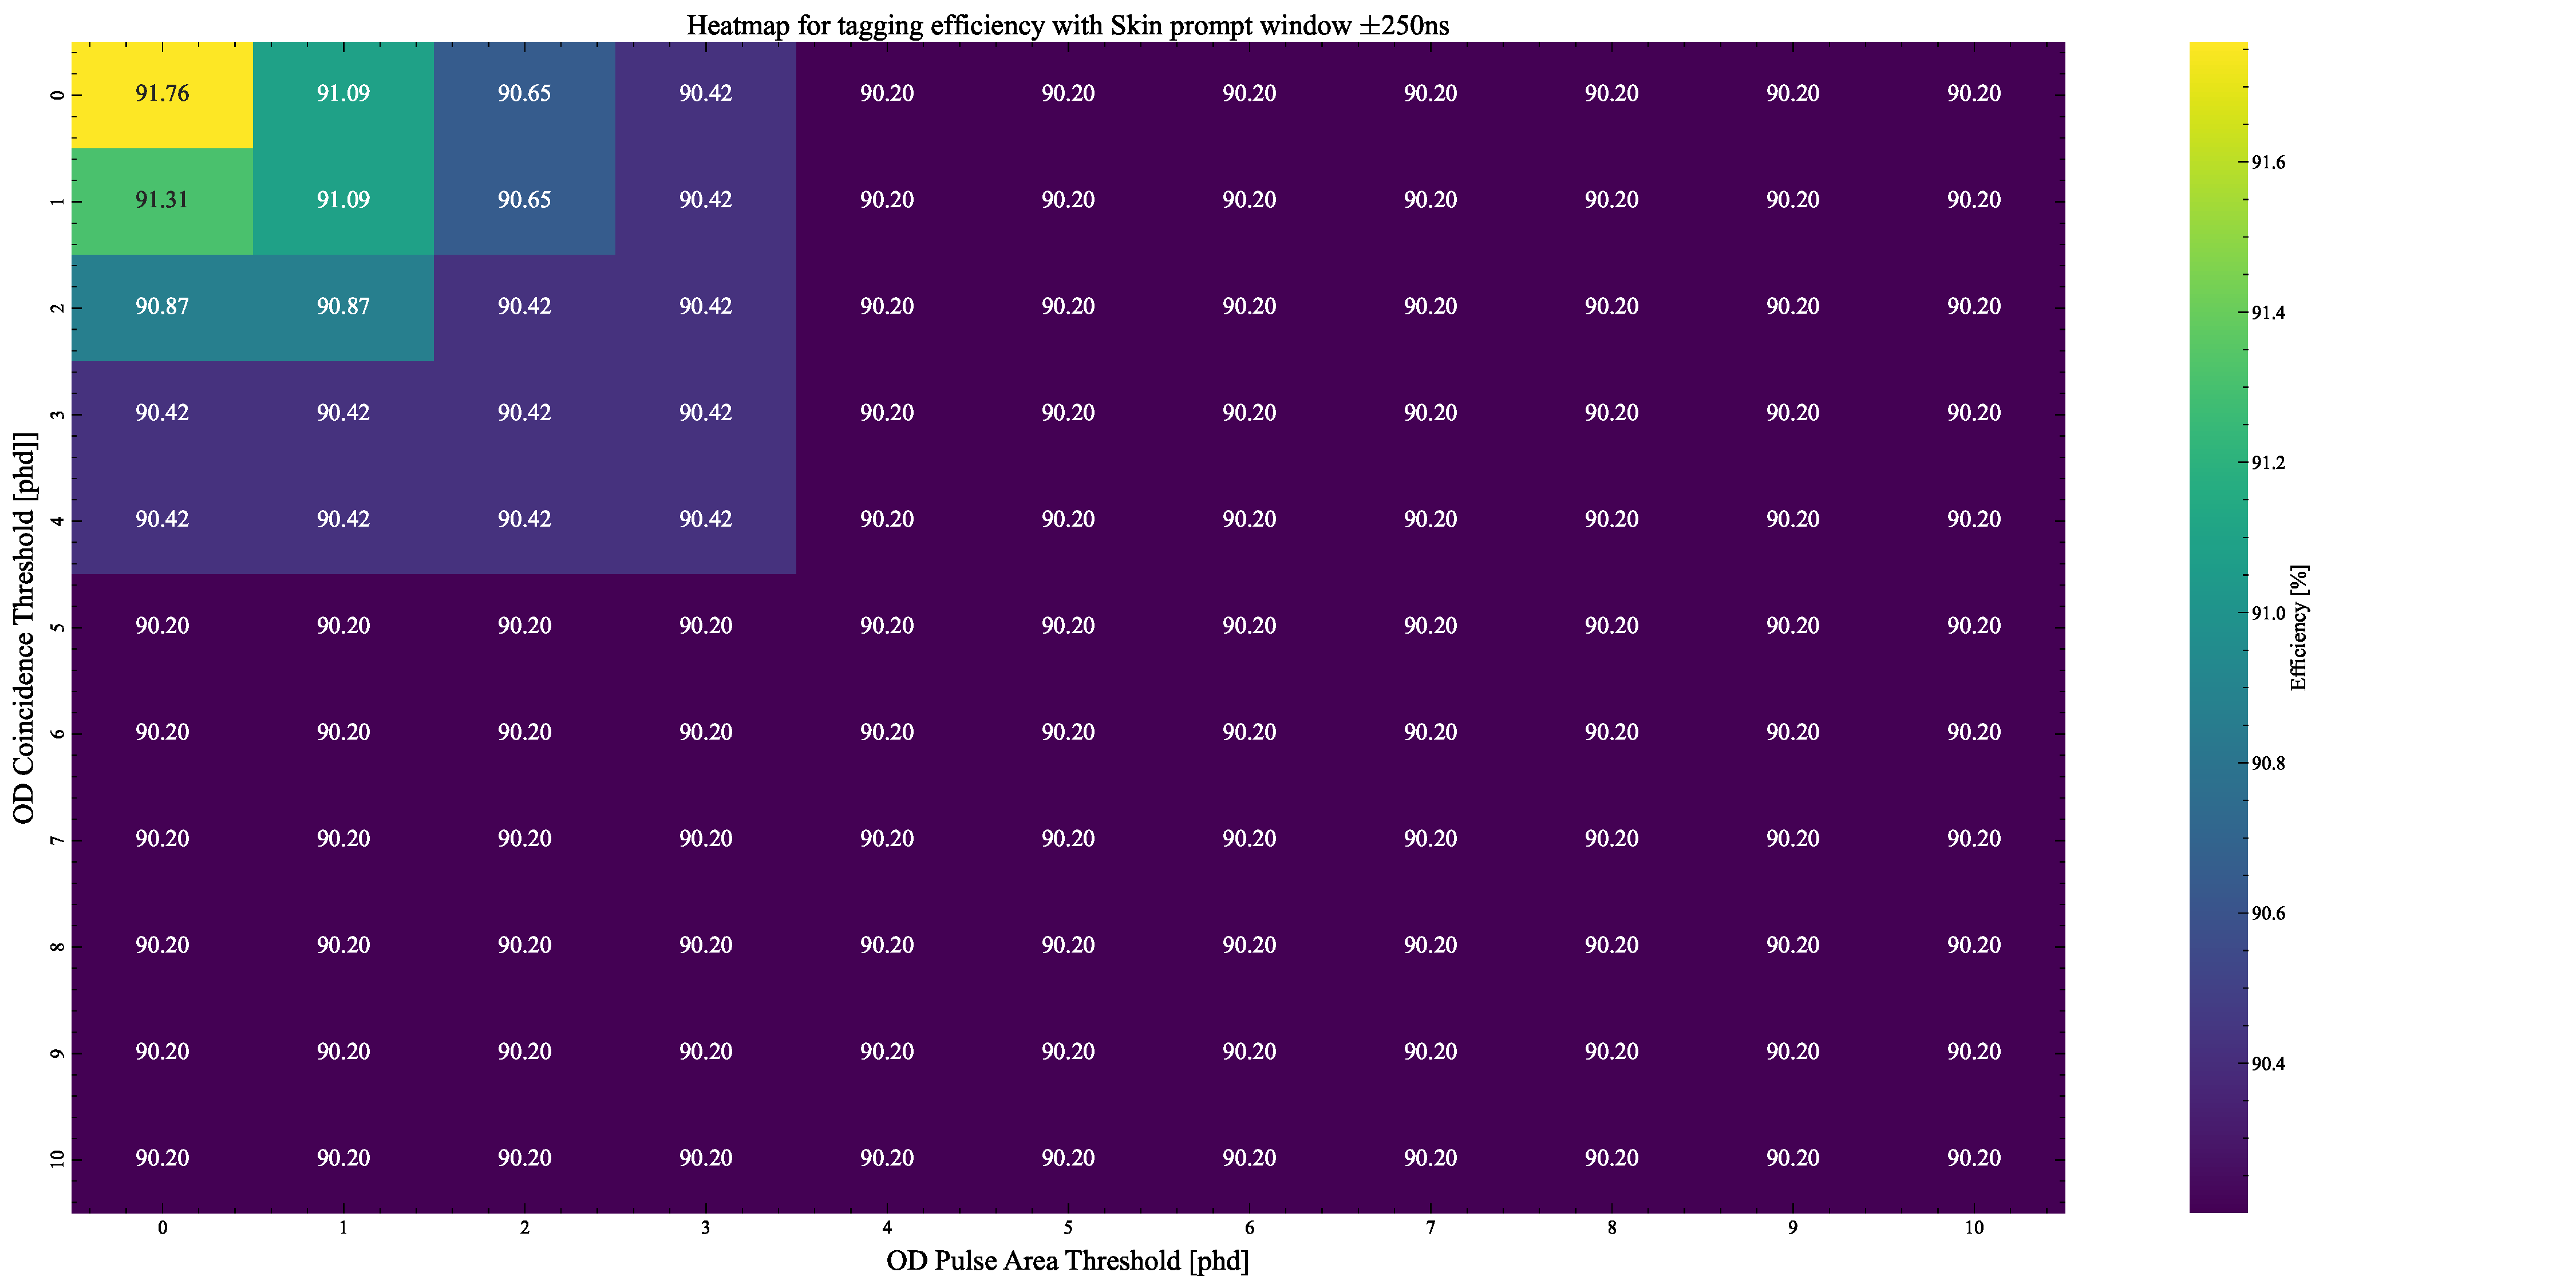
\includegraphics[width=\textwidth]{figures/VetoEfficiency/HeatmapSkinPACoinScanWindow500.pdf}
    \caption{Skin Prompt heatmap.
    In each bin, either the pulse coincidence or the pulse threshold has been varied.
    The z-axis shows the efficiency associated with a given pulse requirement.
    The veto time window considered is [-250, 250]ns.}
    \label{fig:skin_prompt_veto_heatmap}
\end{sidewaysfigure}
\begin{sidewaysfigure}
    \centering
    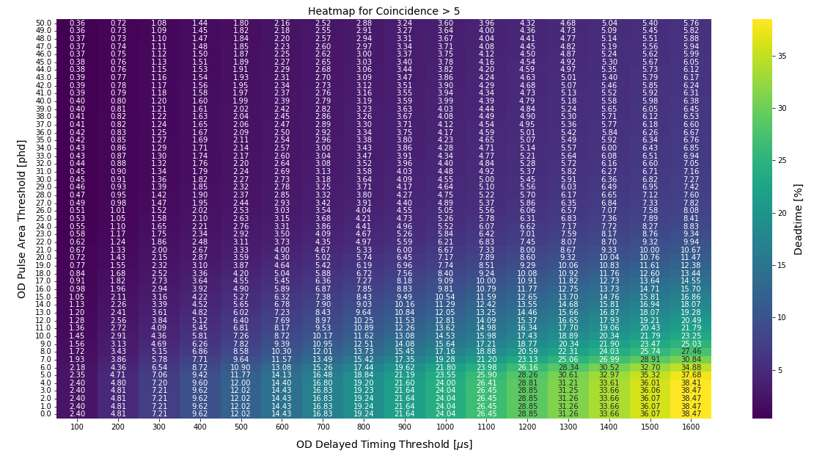
\includegraphics[width=\textwidth]{figures/VetoEfficiency/HeatMapOD_PA_ScanWindow_deadtime.png}
    \caption{OD Delayed heatmap.
    In each bin, either the veto window or the pulse threshold has been varied.
    The z-axis shows the deadtime associated with a given veto window and pulse threshold.
    In addition to the pulse area threshold, the pulse must have a coincidence greater than 5.}
    \label{fig:od_delayed_veto_heatmap}
\end{sidewaysfigure}
\begin{sidewaysfigure}
    \centering
    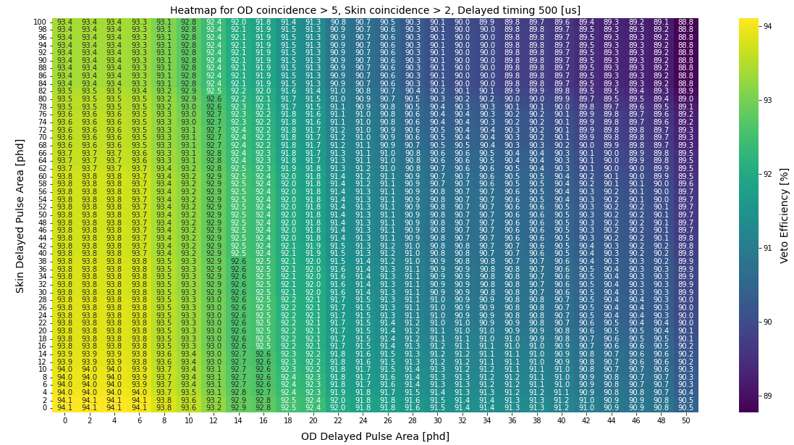
\includegraphics[width=\textwidth]{figures/VetoEfficiency/HeatMap_ODPA_SkinPA_eff.png}
    \caption{Delayed vetoes heatmap.
    In each bin, the OD pulse threshold or the Skin pulse threshold has been varied.
    The z-axis shows the veto efficiency associated with a given pulse thresholds.
    In addition to the pulse area threshold, the OD pulse must have a coincidence greater than 5, and the Skin pulse greater than 2.
    The veto window in this case is 500$\mu$s.}
    \label{fig:skin_delayed_veto_heatmap}
\end{sidewaysfigure}

\begin{figure}
    \centering
    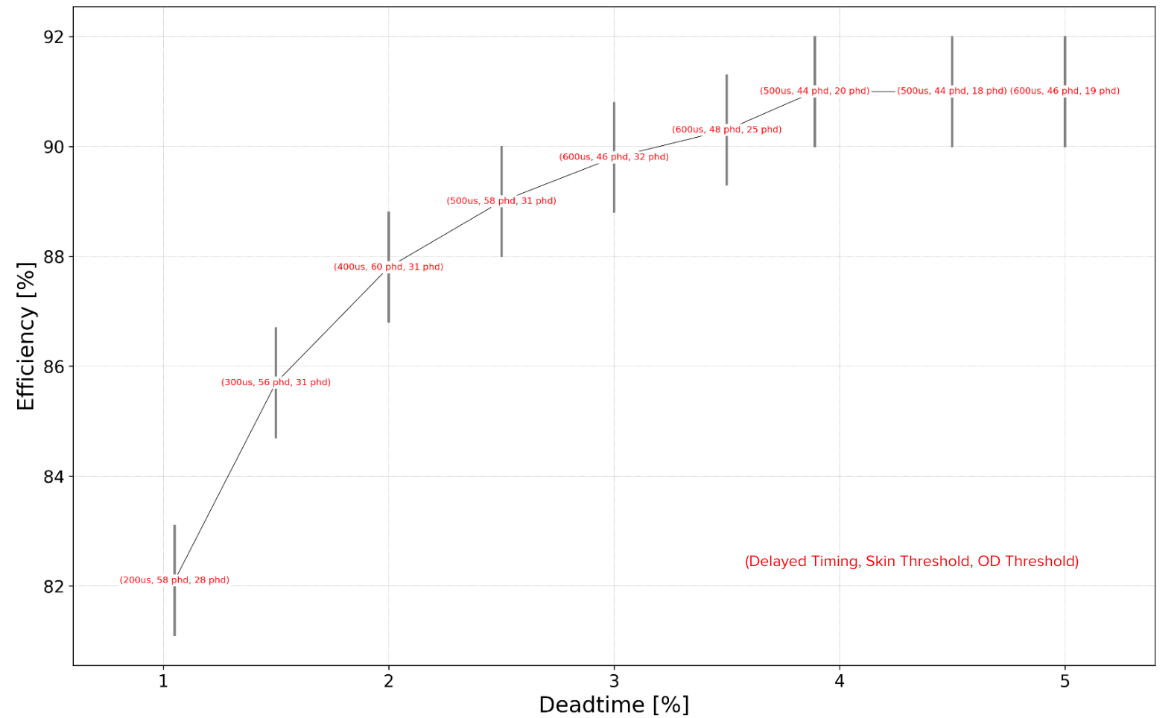
\includegraphics[width=0.9\textwidth]{figures/VetoEfficiency/cut_optimisation.png}
    \caption{Deadtime-vs-efficiency highlighting a number of considered cuts.
    At each point, the numbers in brackets are; the delayed veto window length after the TPC single-scatter, the Skin threshold pulse area, and the OD threshold pulse area.}
    \label{fig:veto_cut_optimisation}
\end{figure}

\begin{figure}
    \centering
    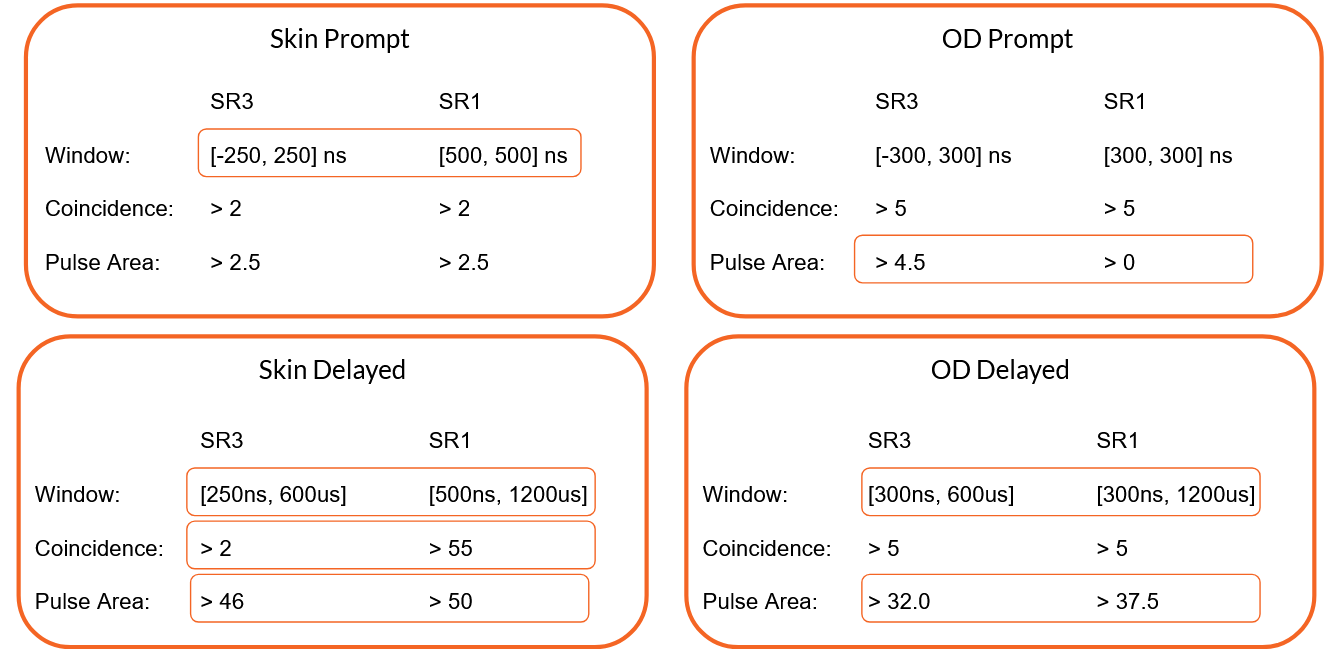
\includegraphics[width=0.9\textwidth]{figures/VetoEfficiency/sr3_cuts.png}
    \caption{Cuts determined to be optimal for SR3. 
    The SR3 thresholds have a position correction in Z. The SR1 cuts are also included.}
    \label{fig:sr3_veto_cuts}
\end{figure}

\subsection{Deadtime Stability}

The deadtime for each of the veto cuts was checked that it is stable over SR3.
This was done by breaking up the SR3-WS file list, in this case, \textbf{SR3-WSv7-LZAP-5.8.0}, into month-by-month chunks.
On each month, the rate of pulses in the Skin and OD from the second half of Random Trigger data was used; and the rate above threshold - where the threshold is the veto cut - is recorded. The stability of this over SR3 is shown in \autoref{fig:deadtime_stability}.

The deadtime is then calculated as;
\begin{equation}
    \textrm{Dead Time [\%]} = 1 - e^{-\lambda (x)}
\end{equation}
where $\lambda$ is the background rate and $x$, the veto threshold.
%The deadtime can also be approximated by;
%\begin{equation}
%    \textrm{Approx. Dead Time [\%]} = \textrm{Rate of events above threshold [Hz]} \times \textrm{Veto window length [s]} \times 100
%\end{equation}

The conclusion that the dead-time is stable over SR3 was also checked by looking at the \lstinline{ODHealth} PREM module, shown in \autoref{fig:deadtime_stability_prem}.
The PREM module shows the rate of OD pulses above $200~keV$ (as defined by the SR1-$200~keV$ not from the SR3 energy calibration), with no significant fluctuation during SR3.
\begin{figure}
    \centering
    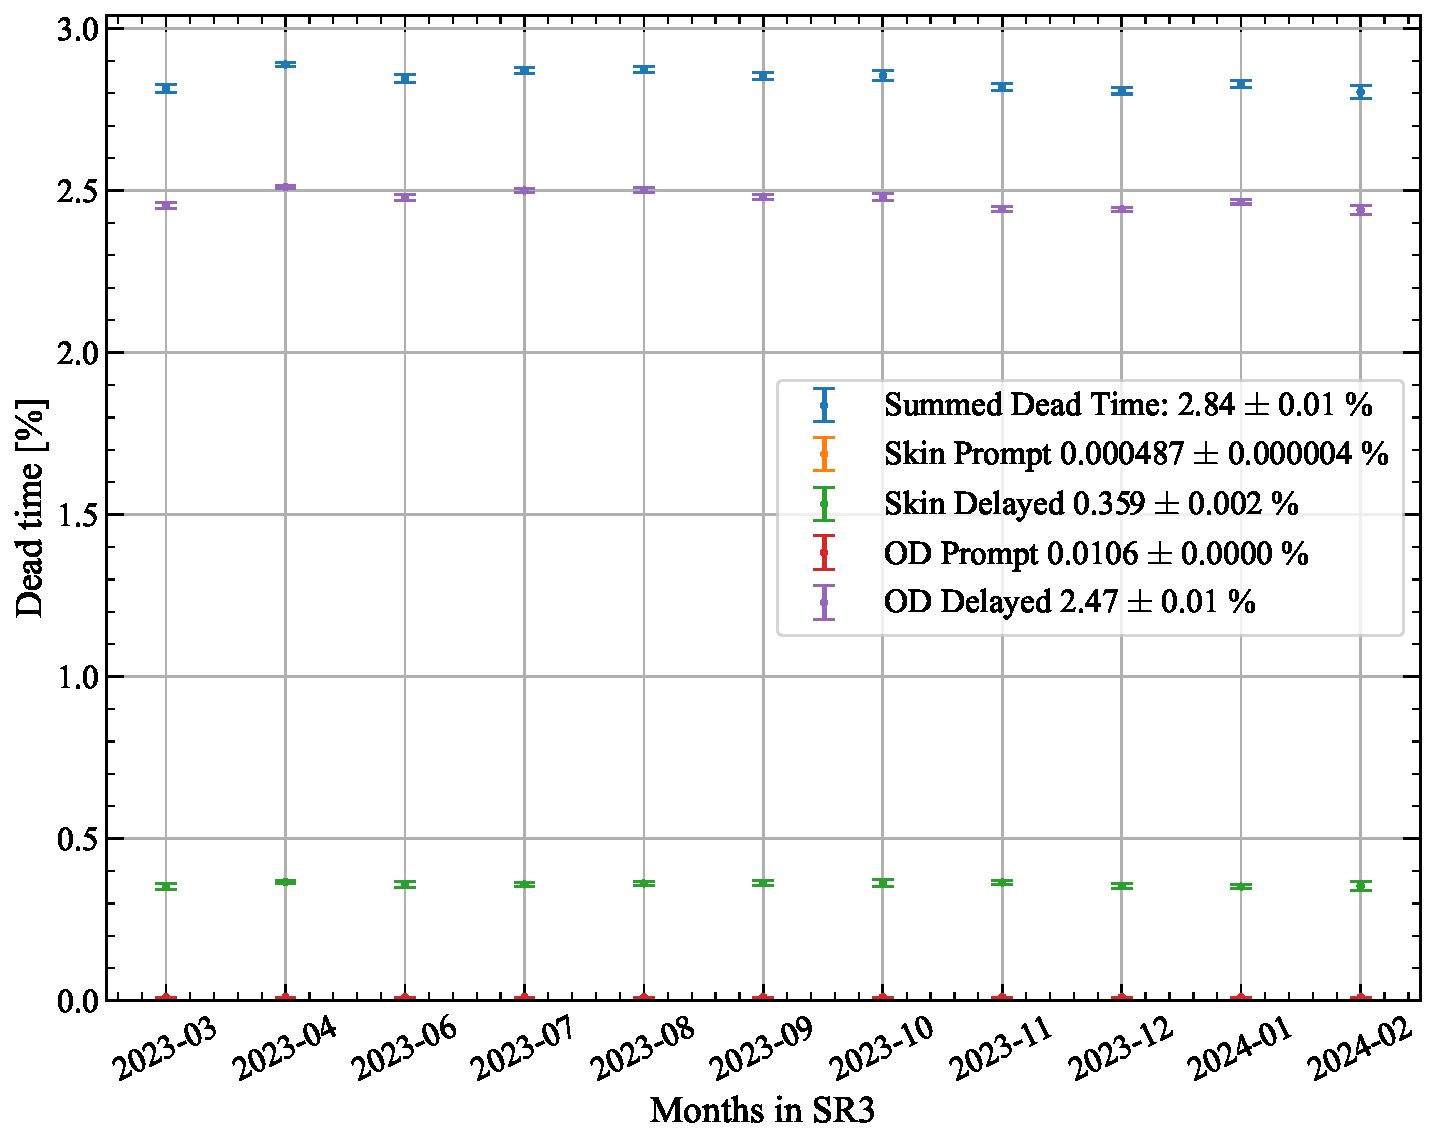
\includegraphics[width=0.7\textwidth]{figures/VetoEfficiency/SR3DeadTimeAll_expoFunc.pdf}
    \caption{Deadtime from the Skin and OD veto cuts during each month of SR3. The error shown in purely statistical.}
    \label{fig:deadtime_stability}
\end{figure}
\begin{figure}
    \centering
    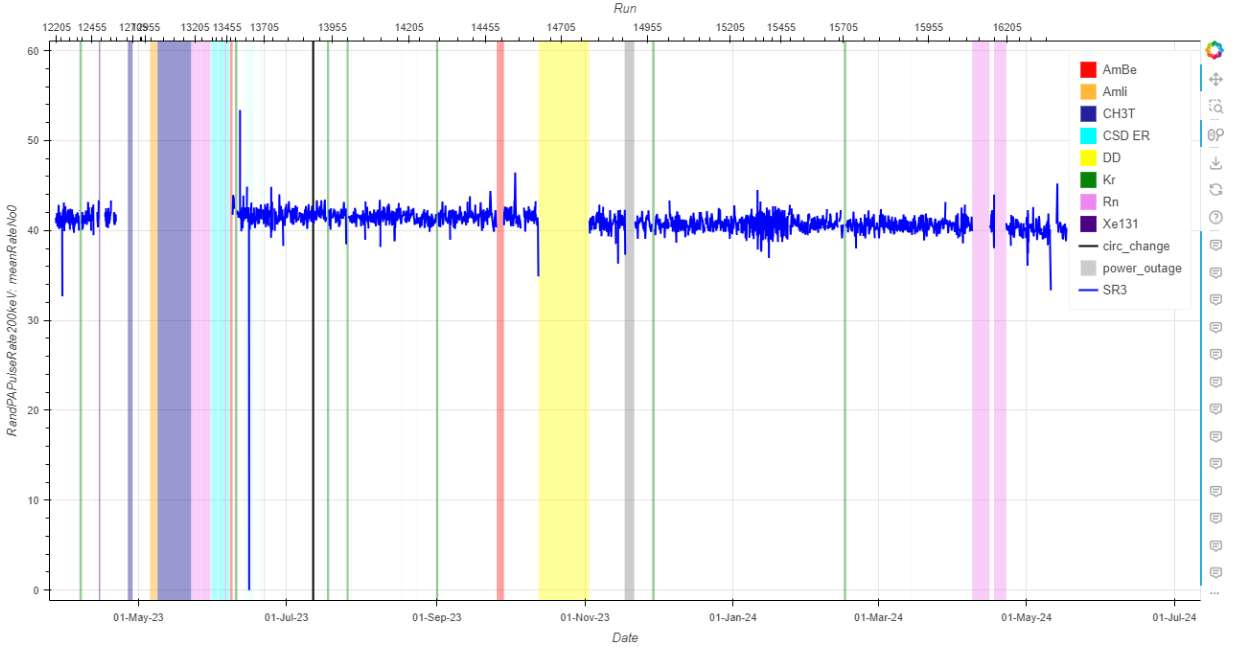
\includegraphics[width=0.7\textwidth]{figures/VetoEfficiency/prem_od_stability.png}
    \caption{Rate of OD pulses above 200keV as defined by SR1 not SR3.}
    \label{fig:deadtime_stability_prem}
\end{figure}

\section{Neutron Veto Efficiency \label{sec:efficiency}}
In this section, the efficiency of tagging background neutrons using the Skin and OD detectors is calculated.
This is performed by calculating the efficiency on AmLi and DD calibration data. 
This is then compared to AmLi and DD simulations.
The difference between these simulations and data are then used to calculate an offset.
The efficiency is then calculated for detector NR simulations and the offset applied (either a subtraction or a scaling, discussed later).
This gives the neutron tagging efficiency for background neutrons.

\subsection{Efficiency Calculation}
The efficiency is defined as;
\begin{equation}
    \epsilon [\%] = \frac{\textrm{N. Events passing Analysis Cuts + Veto Cuts}}{\textrm{N. Events passing Analysis Cuts}} \times 100
    \label{eq:neutron_tagging_efficiency}
\end{equation}
and the inefficiency is defined as $100 - \epsilon$.

\subsection{Neutrons From Calibration Sources \label{sec:AmLi_Efficiency}}
\subsubsection{AmLi} 
The AmLi calibration runs are from the May-2023 calibration period before SR3, with run control operation name \textbf{Amli-B}.
The runs used are; \lstinline{13004-13026}.
All files were processed with \lstinline{LZap-5.8.0}.

On these events, the selection of cuts were applied.
The majority of which are `standard' SR3 cuts which are listed in \autoref{tab:amli_efficiency_cuts}.
In addition to the cuts listed in \autoref{tab:amli_efficiency_cuts}, two other categorises of cuts were applied;
\begin{enumerate}
    \item \lstinline{CSD tube}: This is a circular cut on the reconstructed position of the SS in the TPC so that events from just one CSD tube are selected at a time. To make the comparison between data and simulation this cut is required because in simulation only one source in one tube was simulated as opposed to deploying a source in each CSD tube simultaneously. This is useful for examining the fluctuation in neutron tagging efficiency with $(x,y,z)$. When the efficiency is averaged across different heights and CSD tube, the average can then be replicated in both data and simulation.
    The cut uses the following logic;
    \begin{lstlisting}
    def CSDSelection(x: float, y: float, which_csd: int=1):
        cent_csd_x = [87.6, -43.9, -43.9]
        cent_csd_y = [-0.13, 75.7, -75.7]
        x_el = pow((x-cent_csd_x[which_csd]),2)
        y_el = pow((y-cent_csd_y[which_csd]),2)
        r2_el = x_el + y_el
        return r2_el < 50**2 
    \end{lstlisting}
    How this looks in $(x,y)$ is shown in \autoref{fig:CSDSelection}. 
    A concern of this cut is that events towards the centre of the TPC are excluded. 
    However, the position averaged efficiency when the CSD cut and not is $(88.21\pm1.03)\%$ and  $(88.25\pm1.22)\%$ respectively.
    Across the $600\mu s$ window, there is no greater than $2\%$ difference between when the cut is and isn't applied.
    This comparison can be seen in \autoref{fig:CSDSelectionEffComp}.
    \item \lstinline{NR-band}: This is a 1-, 3-, or 5-$\sigma$ cut around the NR band median. 
    The purpose of this cut is to improve the purity of the selection.
    In this note, the 1-$\sigma$ is used.
    The band can be found on NERSC at \lstinline{/global/cfs/cdirs/lz/physics/NEST_Bands/SR3/20240313/Calibration}, if the band has been, it can be recreated with the Woods parameters listed below;
    \begin{lstlisting}
The Woods Function Fit Parameters for the Band Mean are:  [-6.709932875296116, 7.230400677496497, 0.001868430053684265, 3.648854814073587]
The Woods Function Fit Parameters for the -1 Sigma Line are:  [-7.995805026708432, 7.163090296730374, 0.0018689902999408099, 3.6135843431273336]
The Woods Function Fit Parameters for the +1 Sigma Line are:  [-5.428217339686645, 7.337771458785042, 0.0018671903851709354, 3.684225777881352]
    \end{lstlisting}
    The three different NR bands for the three calibration sources can be seen in \autoref{fig:SR3NRBands}.
    \end{enumerate}

\begin{figure}
            \centering
            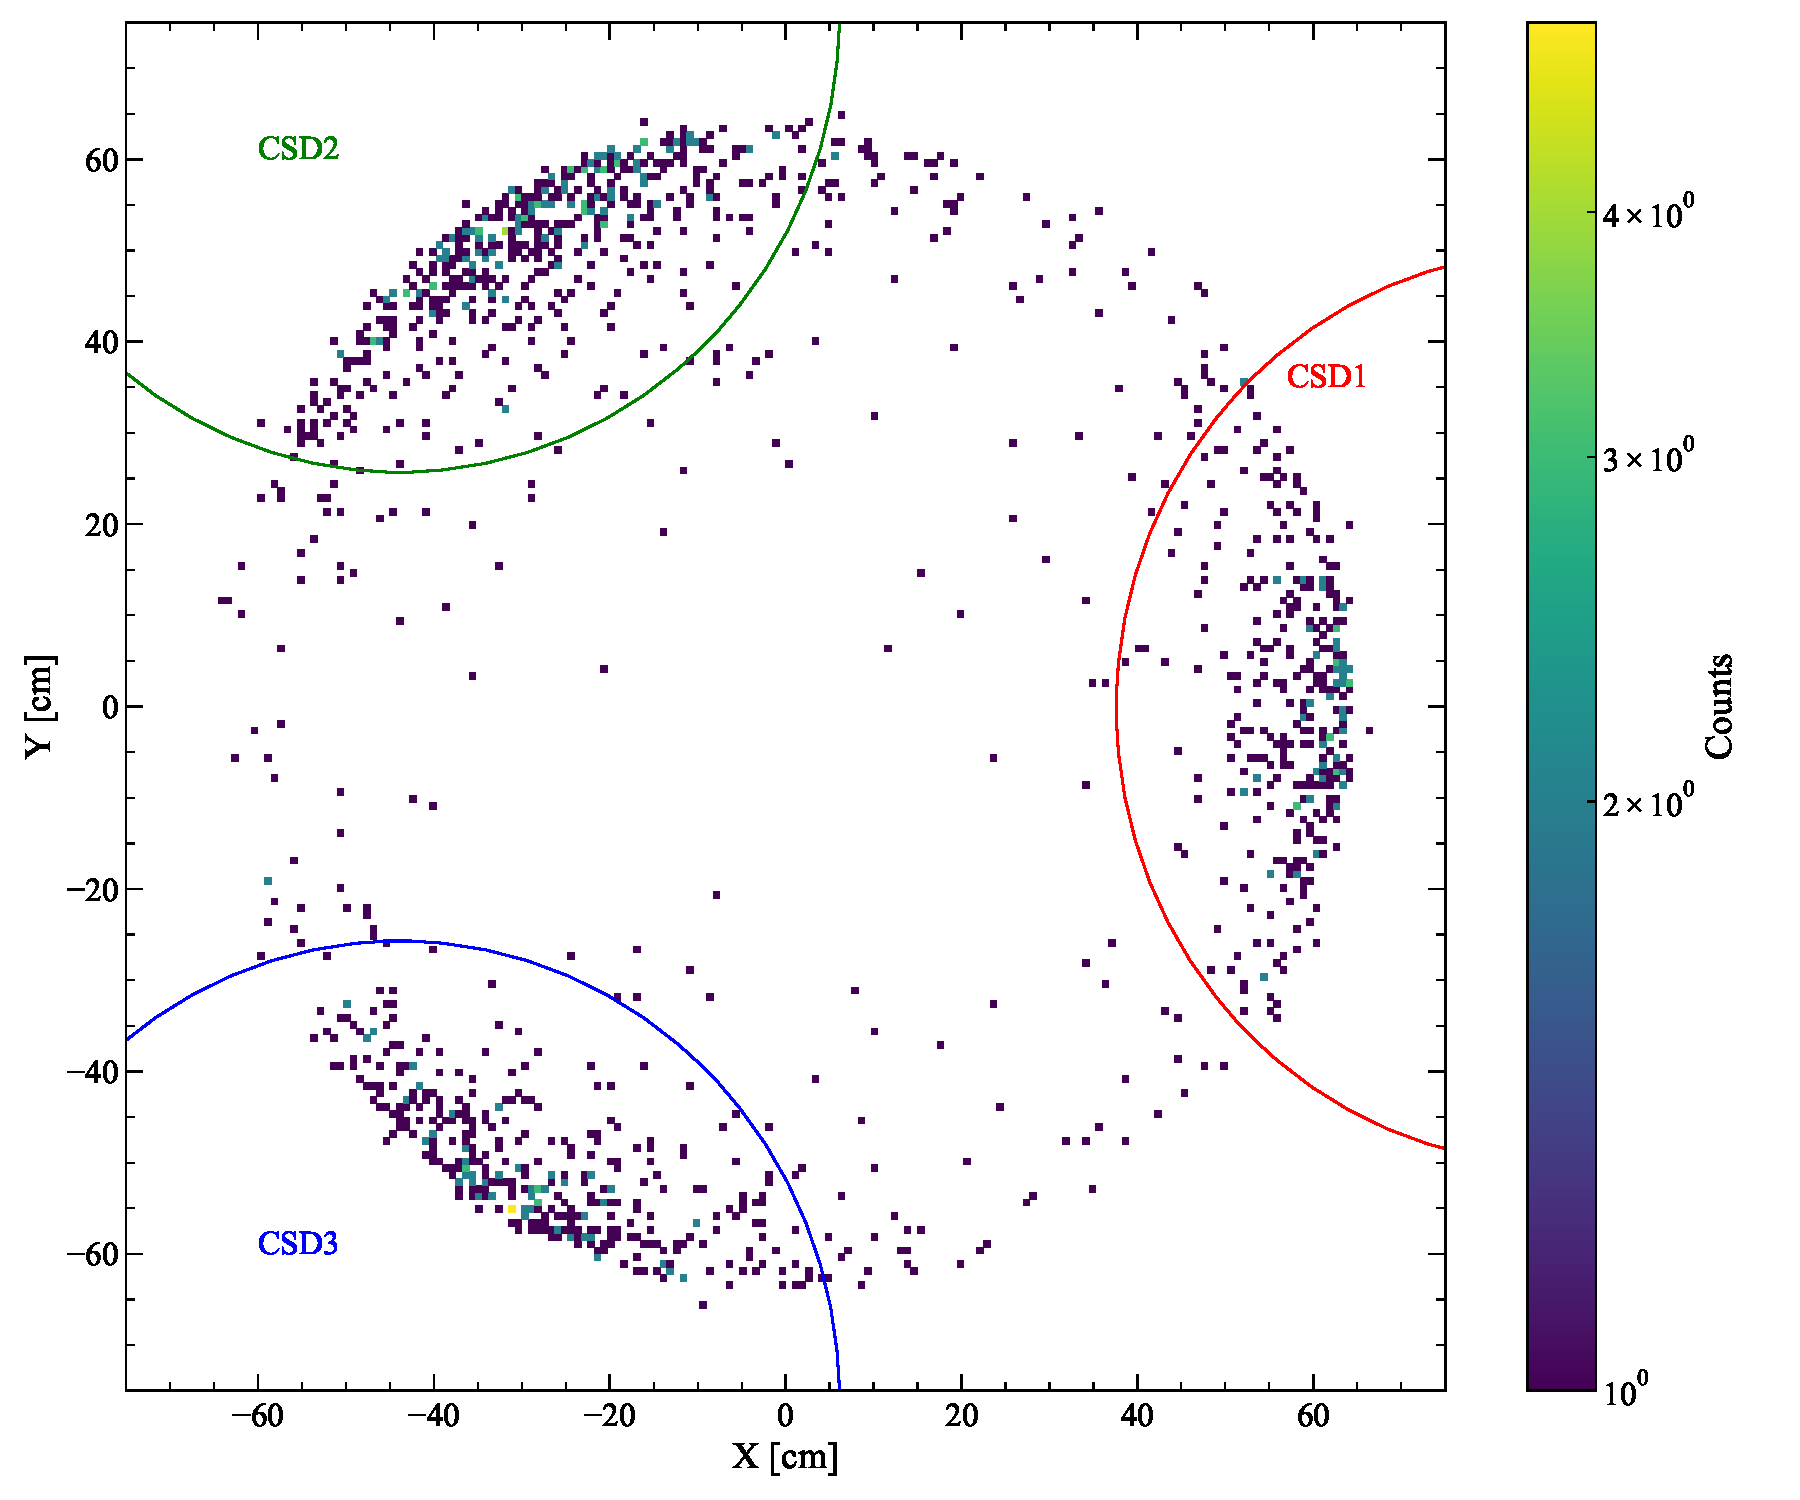
\includegraphics[width=0.5\textwidth]{figures/VetoEfficiency/CircularCSDCut.pdf}
            \caption{X-Y distribution of events in the TPC for AmLi sources positioned at 700mm. Each of the circular cuts are overlaid onto the plot.}
            \label{fig:CSDSelection}
\end{figure}
\begin{figure}
        \centering
        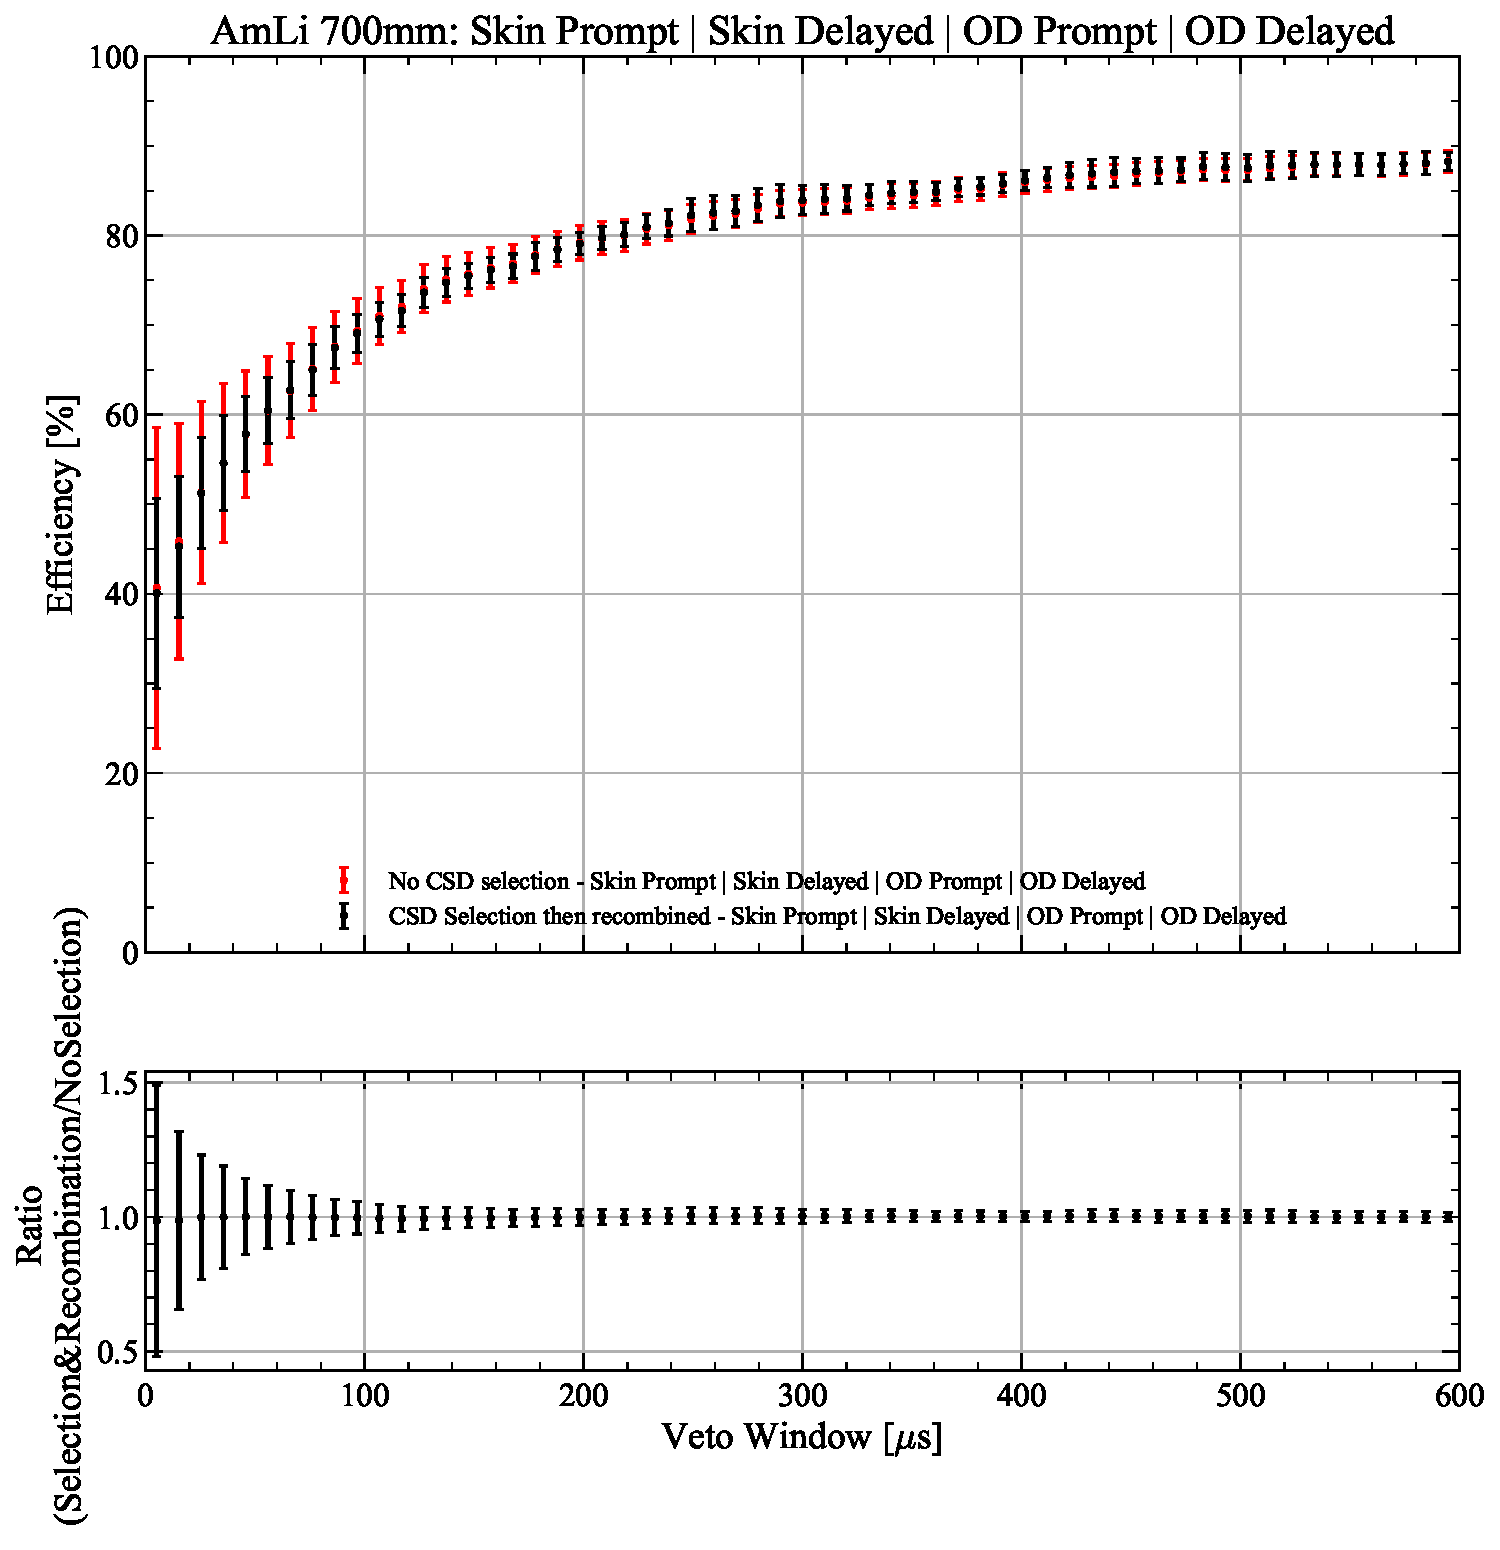
\includegraphics[width=0.5\linewidth]{figures/VetoEfficiency/AmLi_700mm_Total_CSDSelection.pdf}
        \caption{The veto efficiency (from all analysis cuts) at using AmLi at 700mm. The ratio plot shows the less than $2\%$ difference between method 1 and method 2.}
        \label{fig:CSDSelectionEffComp}
\end{figure}
\begin{figure}
            \centering
            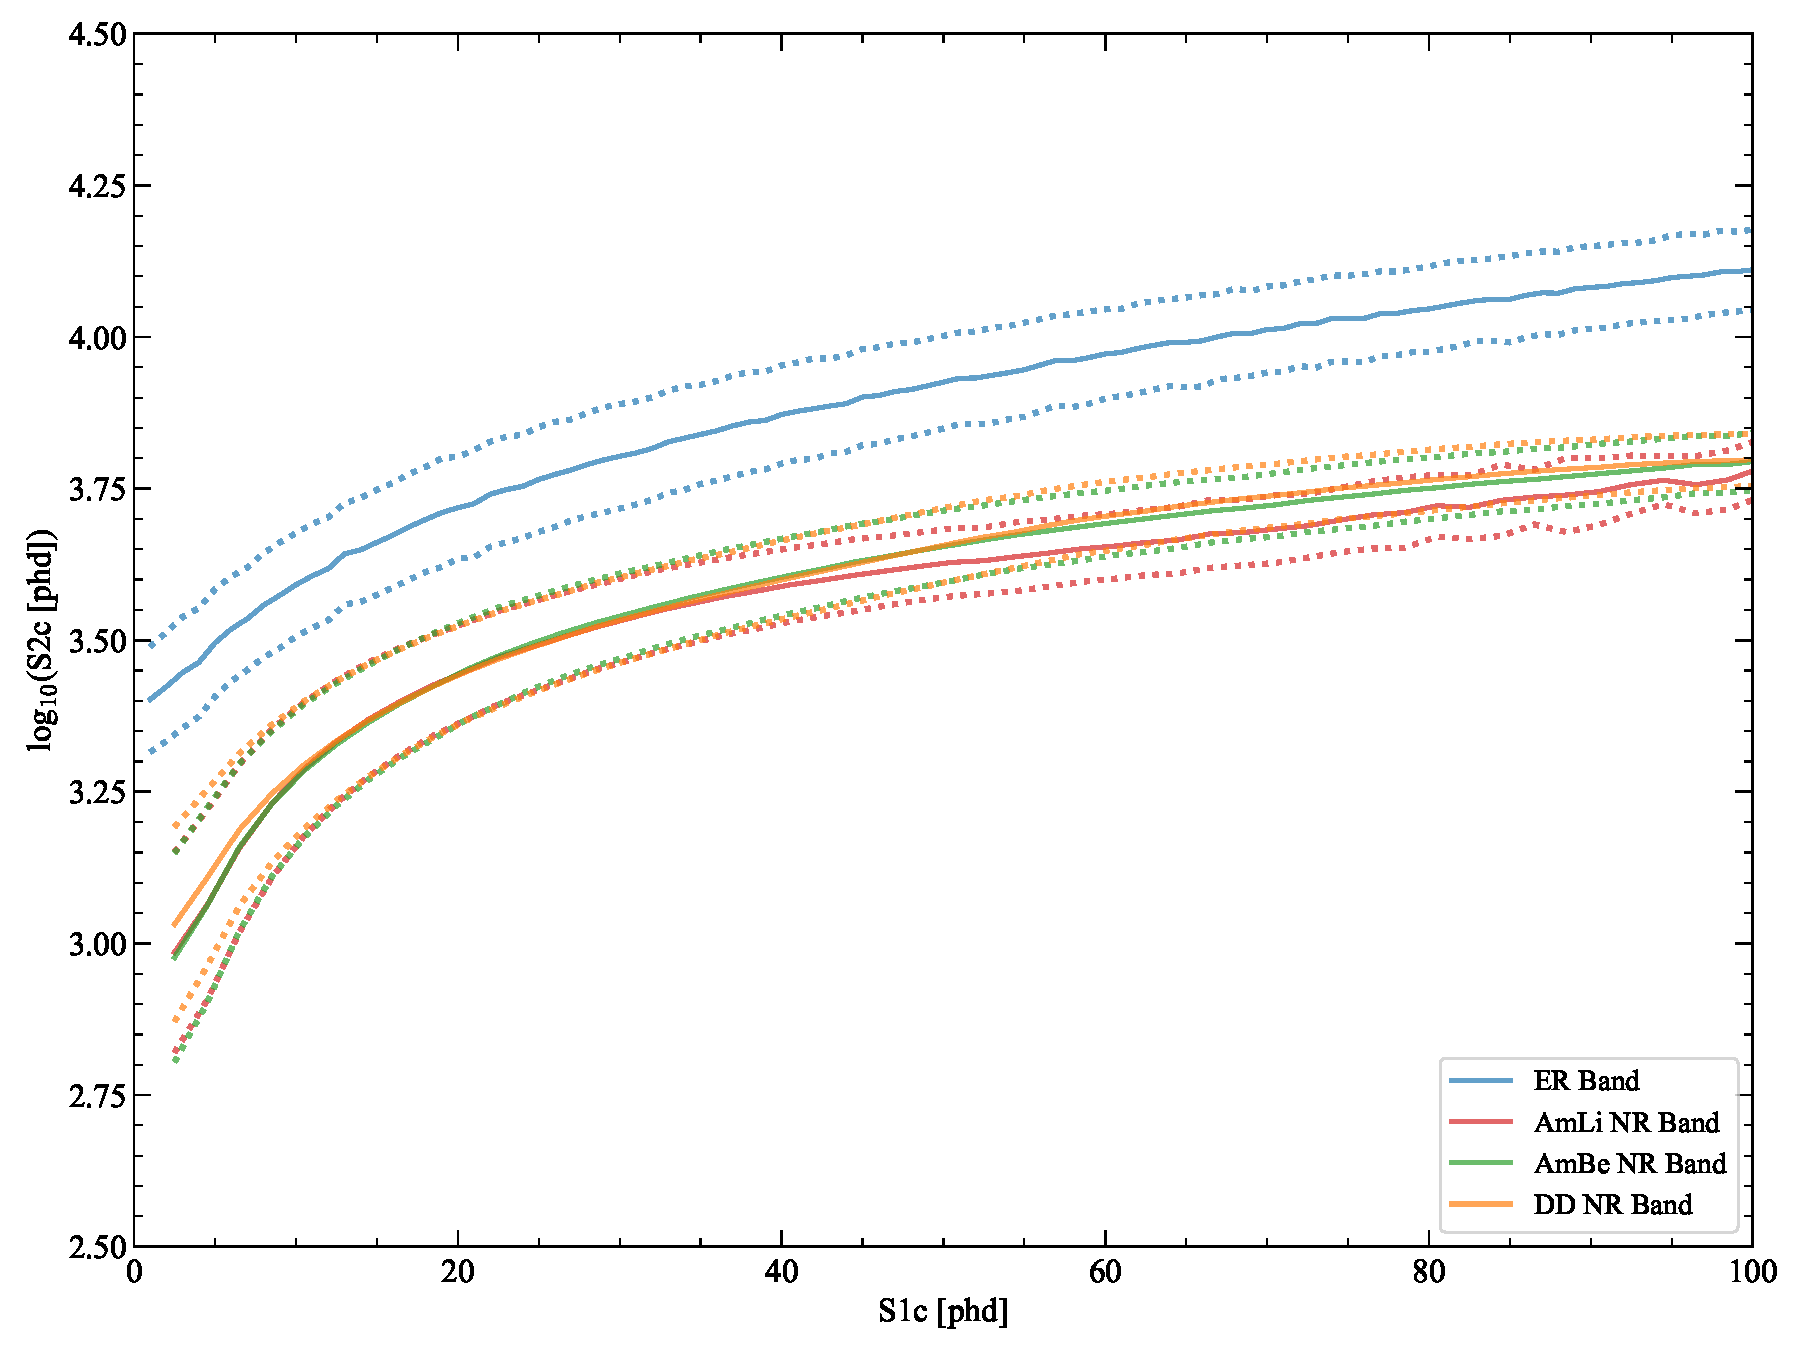
\includegraphics[width=0.8\textwidth]{figures/VetoEfficiency/SR3NRBands.pdf}
            \caption{The three different NR bands used for the NR-band cut for the respective sources, AmLi, DD and AmBe.}
            \label{fig:SR3NRBands}
\end{figure}
\begin{table}
    \centering
    \begin{tabular}{c|c|c|c}
     Livetime cuts & Physics cuts & S1 cuts & S2 cuts  \\
     \hline
     Burst noise cut & Single scatter  & S2 width vs drift time & S1 prominence cut \\
     Muon holdoff       & S1 and S2 threshold & Narrow S2 & Stinger event cut \\
     Sustained rate cut & Fiducial Volume & S2 rise time & S1 TBA vs drift time \\
     High S1 rate exclusion & & S2 early peak & S1 HSC cut \\
     Bad buffer cuts & & S2 XY quality & S1 shape \\
     Excess Area cut & & S2 TBA (above-anode gas) & S1 photon timing \\
    \end{tabular}
    \caption{ALPACA-Core SR3 cuts used on AmLi calibration data for determining the efficiency.
    Each cut is from SR3-cuts-v3.
    }
    \label{tab:amli_efficiency_cuts}
\end{table}



\subsubsection{AmLi Accidental Correction}\label{sec:AmLiAccCorrection}
When determining the veto tagging efficiency a correction must be applied to the measured efficiency to account for the accidental coincidences from AmLi gammas (and neutrons) with single scatter nuclear recoils in the TPC which can artificially enhance the measured tagging efficiency.
First, veto inefficiency must be defined. Every time a single scatter nuclear recoil is observed in the TPC, a veto window is opened, this can be recorded using a counter, $N$ every time this happens. 
If there is no pulse observed in the Skin or the OD that satisfies the veto requirements, this event is not vetoed and recorded using a counter, $M$. Resulting in a total inefficiency, $M/N$, and a total efficiency, $1-M/N$.
The effect of the accidentals be a result of the following process. 
If a neutron enters the TPC, scatters and is not detected by the vetos, the counter $M$ should be iterated but there is an accidental coincidence of a gamma or a neutron from the AmLi sources with the TPC scatter so the count is not iterated. 
The probability of this happening can be written as $1-P_a(0)$, where $P_a(0)$ is the probability of seeing zero accidental pulses in the Skin and OD coincidence windows. 
Using probability and the counters, the true inefficiency is described below,
\begin{gather*}
    M_{observed}=M_{true}-M_{true}(1-P_a(0)) \\
    M_{observed}=M_{true}P_a(0)\rightarrow M_{true}=M_{observed}/P_a(0)\\
    Ineff_{true}=M_{true}/N\;and\;Ineff_{observed}=M_{observed}/N\\
    \Rightarrow Ineff_{true}=Ineff_{observed}/P_a(0)
\end{gather*}
Due to the logic of the inefficiency calculation is that the $M$ counter iterates in an AND condition such that all coincidence windows in all detector have to be empty. 
This leads to a final inefficiency of,
\begin{equation}
    Ineff_{true} = Ineff_{obs}  / (1 - P_a(>0)_{any\:window})
\end{equation}
$P_a(>0)_{any\:window}$ can be determined directly using the post-trigger window of randomly triggered events (GPS events) and count any pulses in \textbf{any} of the veto detectors. 
The accidental correction is correlated with the length of the veto window, scans over the entire delayed veto window in 10$\mu$s steps, the change in the correction factor over time can be seen in \autoref{fig:AccCorr}.
The impact of the accidental correction when applied to the efficiency can be seen in \autoref{fig:AccidentalImpact}.

\begin{figure}
    \centering
    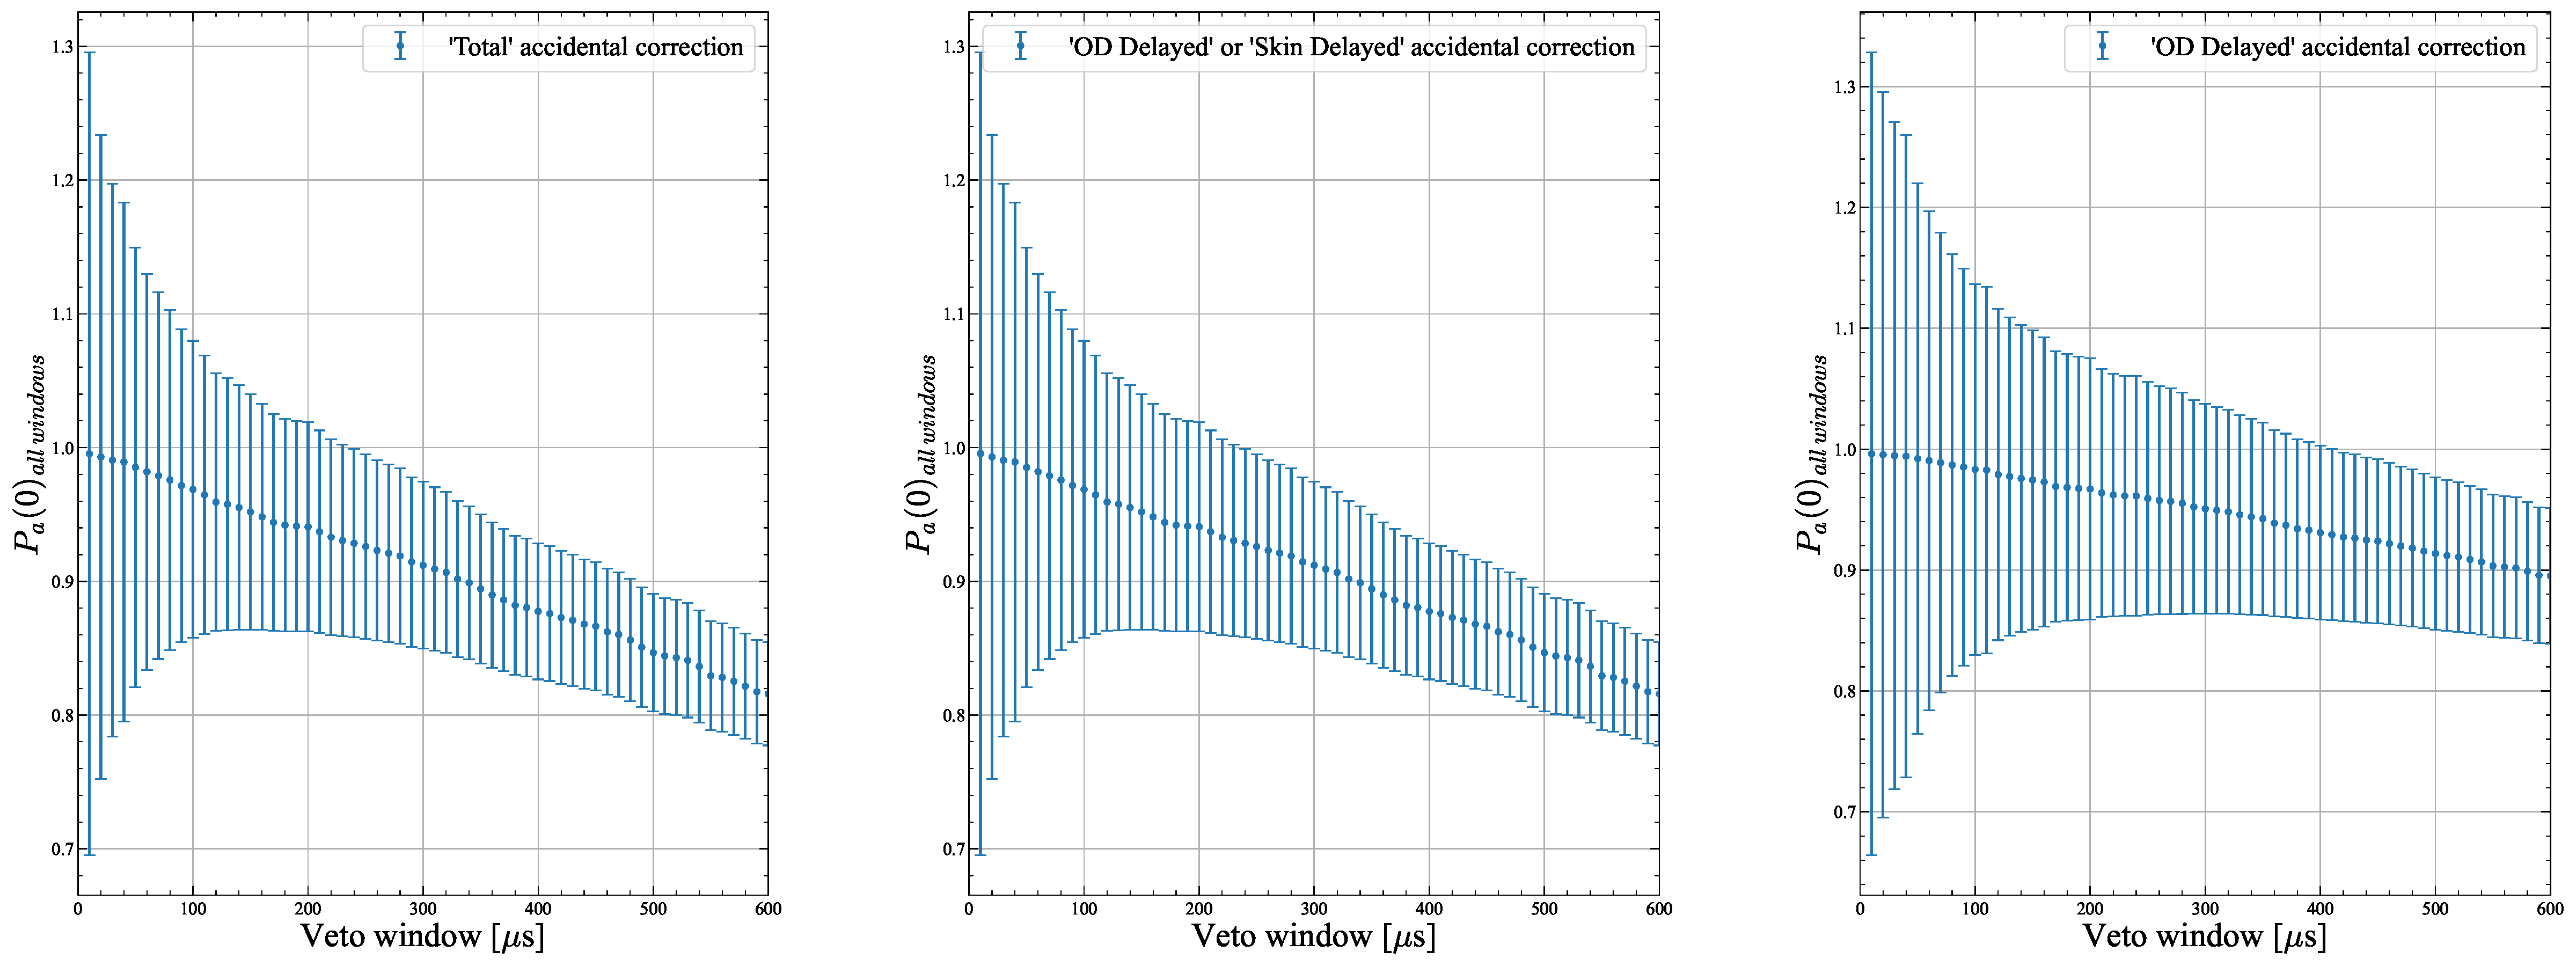
\includegraphics[width=\textwidth]{figures/VetoEfficiency/SR3AmLi_700_Corrections_100k_P0.pdf}
    \caption{$P_a(>0)_{all\:window}$ AmLi Accidental correction factors for varying veto window size for different windows of interest.}
    \label{fig:AccCorr}
\end{figure}

\begin{figure}
    \centering
    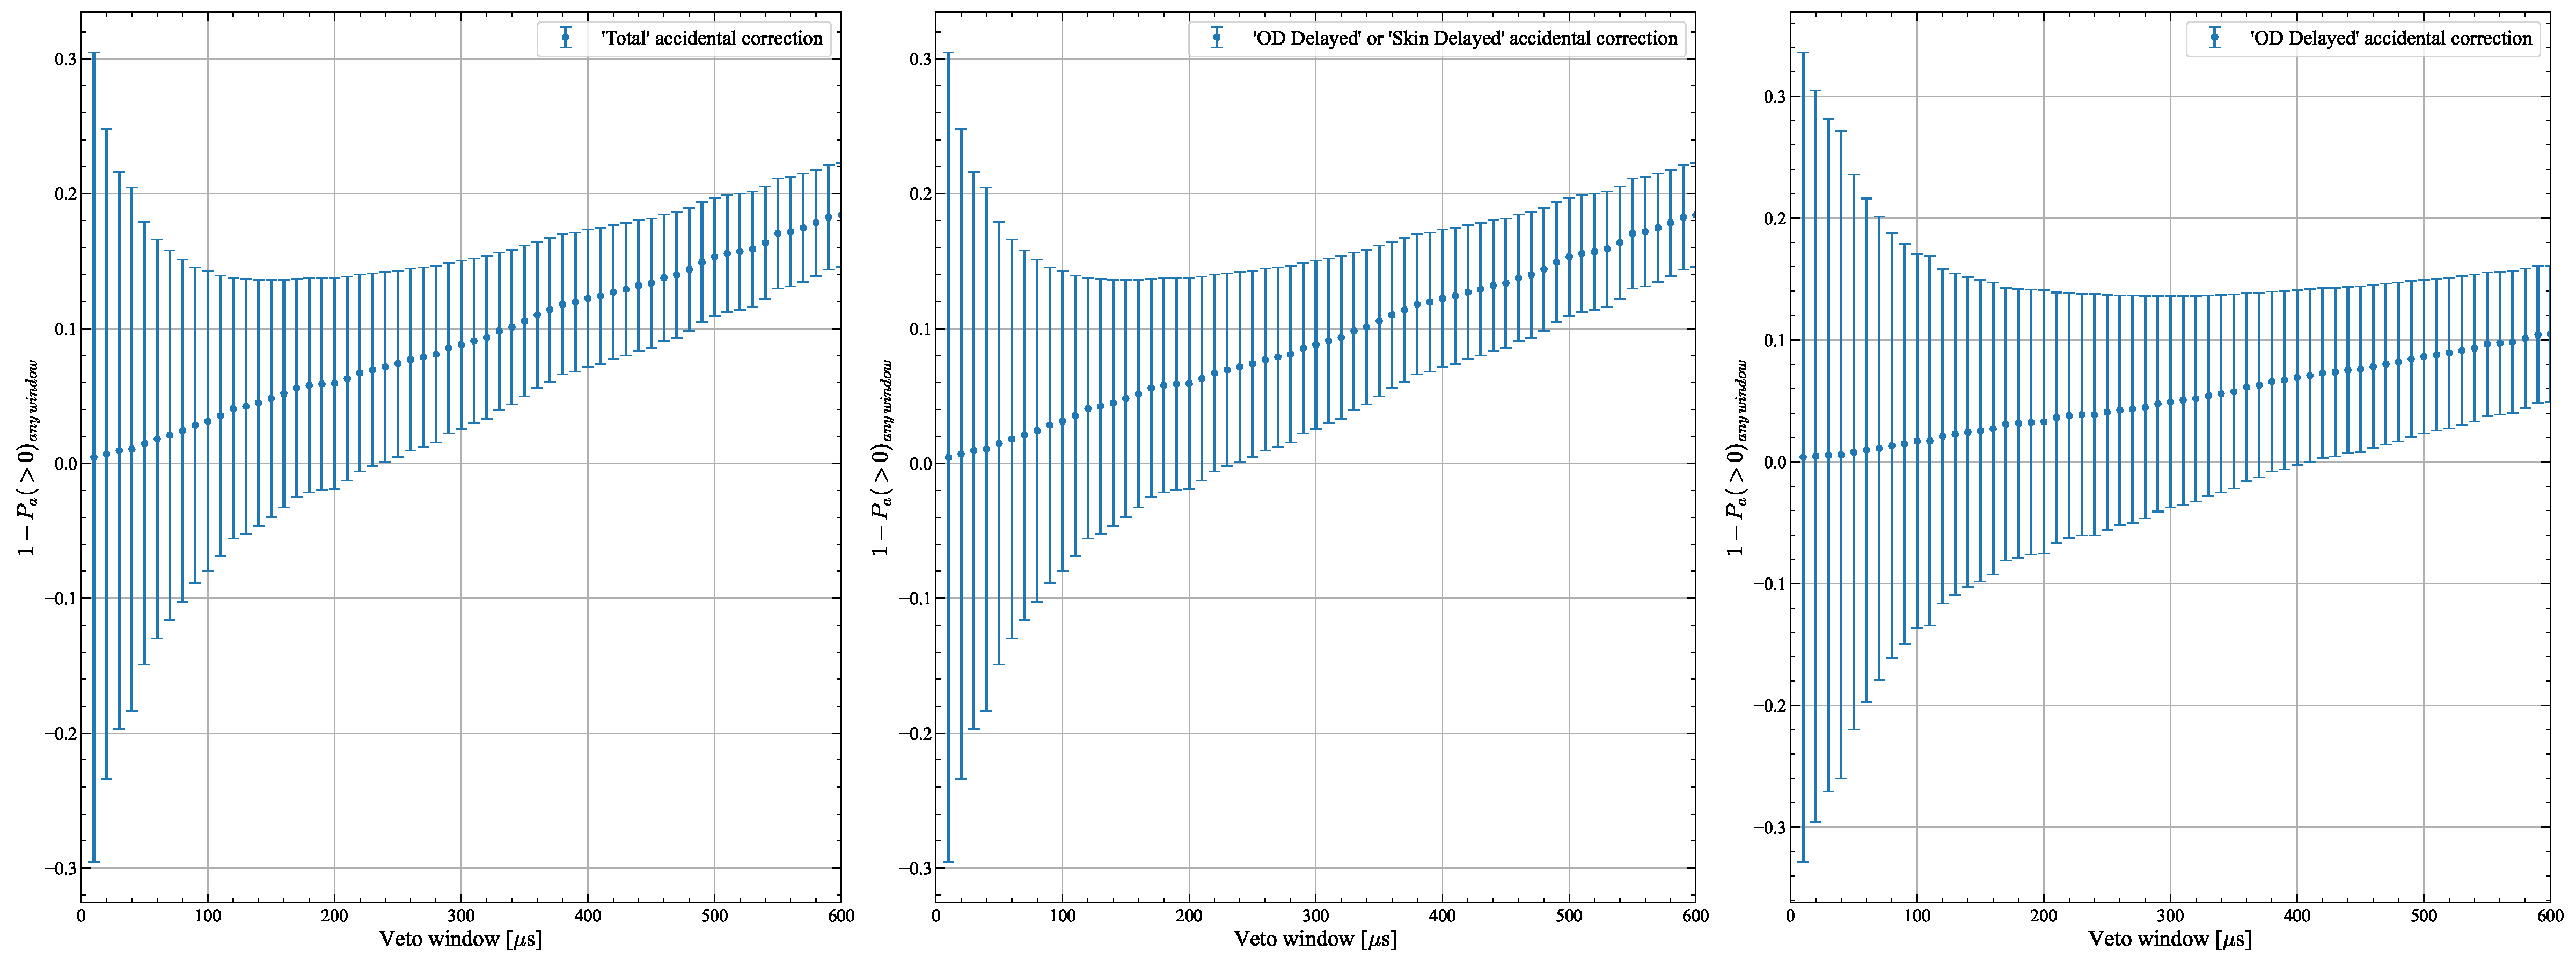
\includegraphics[width=\textwidth]{figures/VetoEfficiency/SR3AmLi_700_Corrections_100k_P0-1.pdf}
    \caption{$1 - P_a(>0)_{any window}$ AmLi Accidental correction factors for varying veto window size for different windows of interest.}
    \label{fig:AccCorr_P0-1}
\end{figure}

\begin{figure}
    \centering
    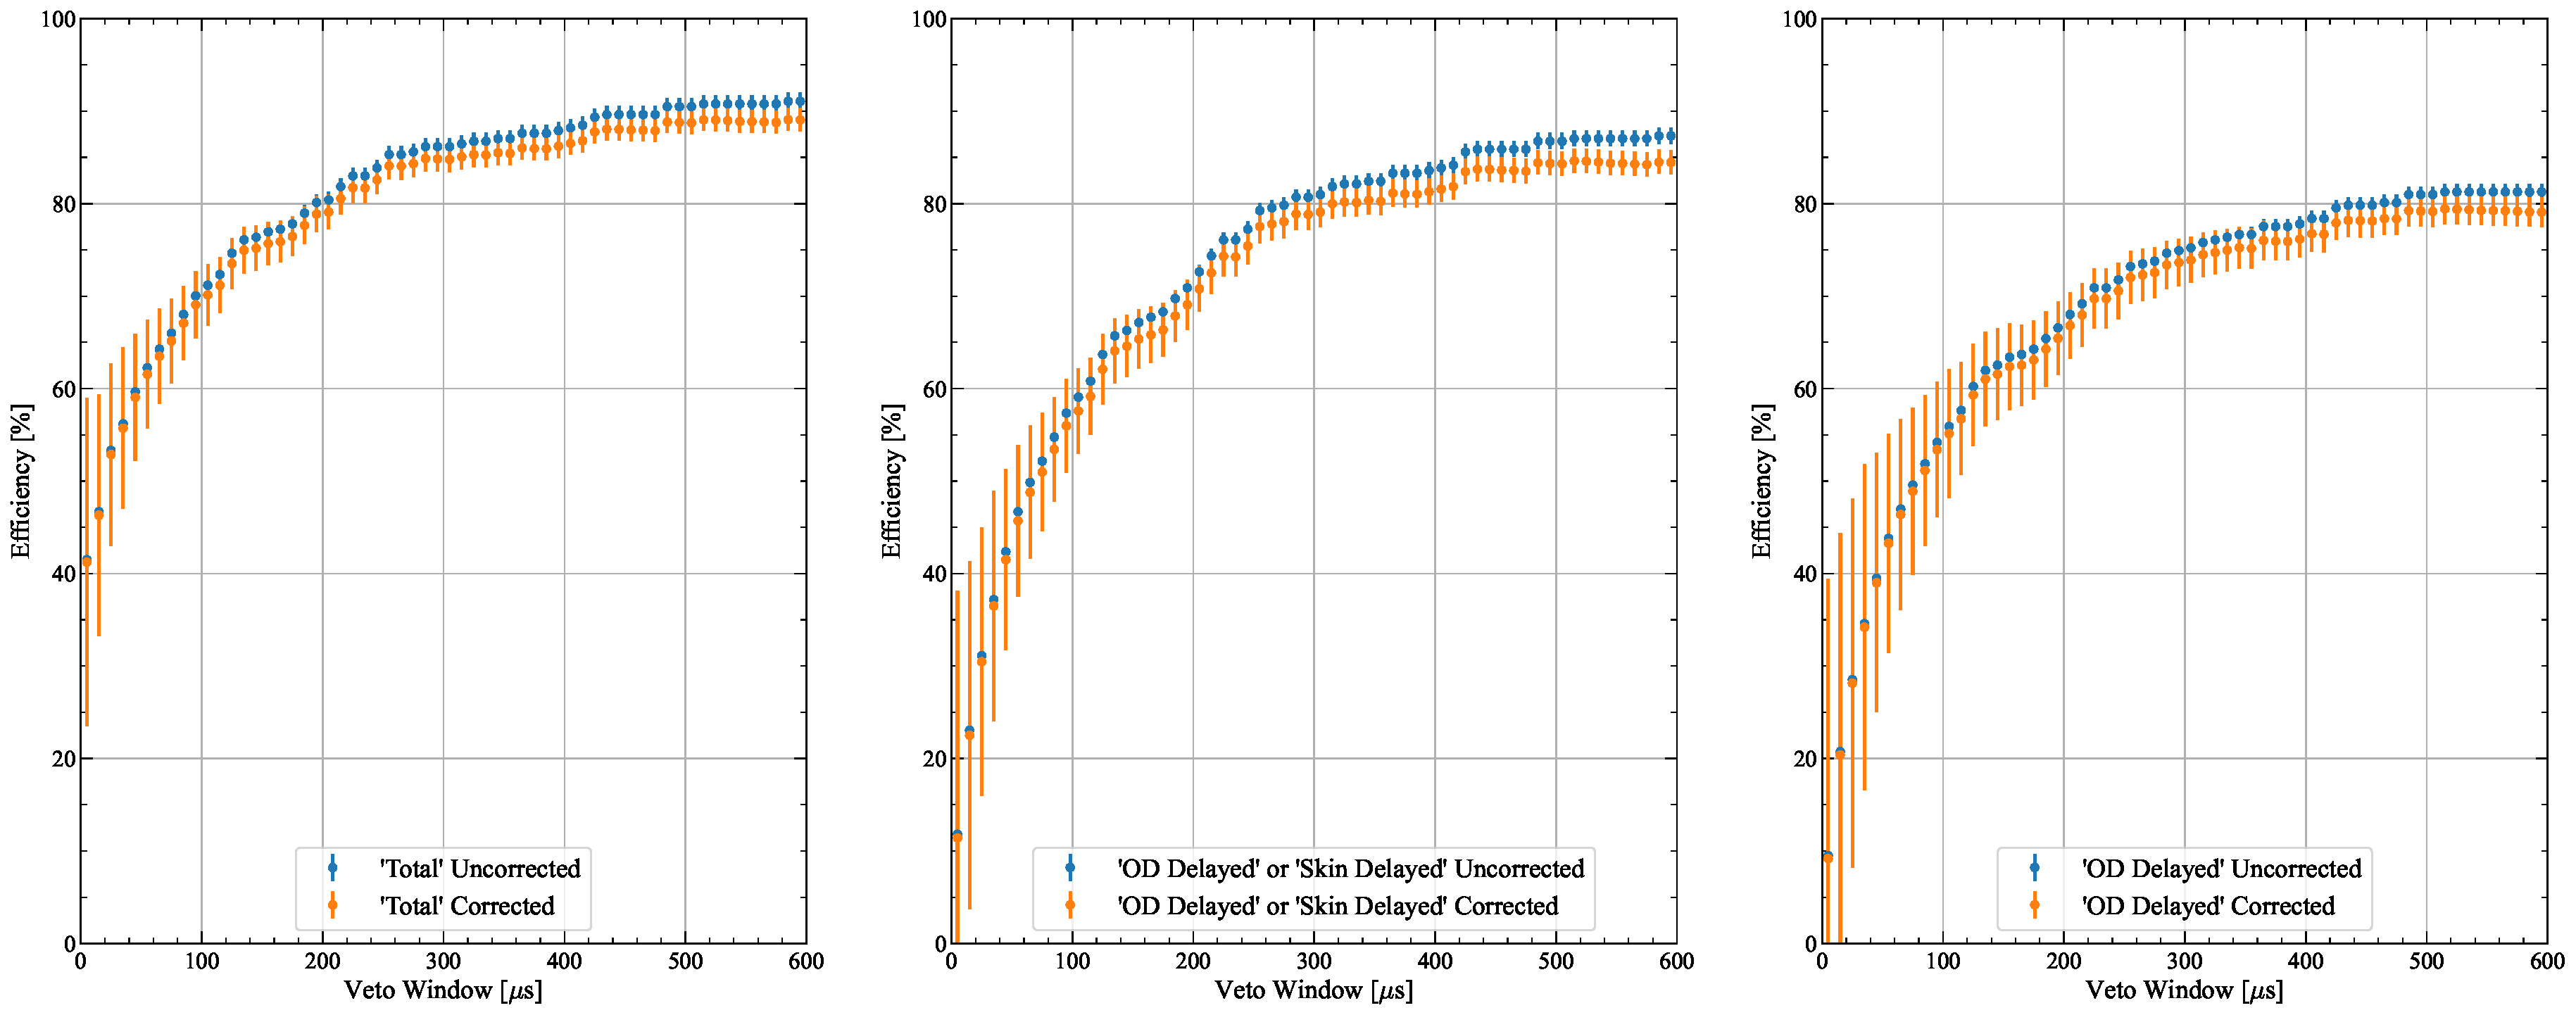
\includegraphics[width=\textwidth]{figures/VetoEfficiency/AccidentalCorrectionImpact.pdf}
    \caption{The impact of the accidental correction applied to the different veto efficiencies for the given windows of interest. AmLi data at a height of 700~mm in CSD1 has been used here as an example.}
    \label{fig:AccidentalImpact}
\end{figure}


\subsubsection{DD Direct}
The DD calibration runs are from the October-2023 calibration period during SR3, with run control operation name \textbf{DD Plasma}.
The runs used are; \lstinline{14631-14654}.
All files were processed with \lstinline{LZap-5.8.0}.

The analysis for DD follows a logic similar to the AmLi described in \autoref{sec:AmLi_Efficiency}.
The cuts used for DD are listed in \autoref{tab:dd_efficiency_cuts}.
In addition to these cuts, an NR band cut was also applied. 
It is important to note that this NR band is different to the one used for AmLi. The three different NR bands for the three calibration sources can be seen in \autoref{fig:SR3NRBands}.
The band can be found on NERSC at \lstinline{/global/cfs/cdirs/lz/physics/NEST_Bands/SR3/20240313/Calibration}, if it has been moved, it can be recreated with the Woods parameters listed below;
\begin{lstlisting}
The Woods Function Fit Parameters for the Band Mean are:  [-19.937161961102728, 19.923601138859933, 0.0003111152850489644, 3.9306761416517557]
The Woods Function Fit Parameters for the 10% CL Line are:  [-17.635537023159518, 15.192184130700792, 0.000791717641575967, 3.813184578175848]
The Woods Function Fit Parameters for the 90% CL Line are:  [-32.02840007751605, 32.68367426603315, -0.0006477294838326959, 4.157363202993382]
\end{lstlisting}
\begin{table}
    \centering
    \begin{tabular}{c|c|c}
     Physics cuts & S1 cuts & S2 cuts  \\
     \hline
     Single scatter  & S2 width vs drift time & S1 prominence cut \\
     S1 and S2 threshold & Narrow S2 & Stinger event cut \\
     Fiducial Volume & S2 rise time & S1 TBA vs drift time \\
     & S2 early peak & S1 HSC cut \\
     & S2 XY quality & S1 shape \\
     & S2 TBA (above-anode gas) & S1 photon timing \\
    \end{tabular}
    \caption{ALPACA-Core SR3 cuts used on DD calibration data for determining the efficiency.
    Each cut is from SR3-cuts-v3.
    }
    \label{tab:dd_efficiency_cuts}
\end{table}
\subsubsection{DD Accidental Correction}
The DD calibration data was also corrected for accidentals. The same method was used which was previously discussed in \autoref{sec:AmLiAccCorrection}. The correction factors used as a function of veto window can be seen in \autoref{fig:figures/VetoEfficiency/DDAccCorrectionParameters}. 
The impact of the accidental corrections on the DD veto efficiency can be seen in \autoref{fig:DDAccCorrectionImpact_P0}.

\begin{figure}
    \centering
    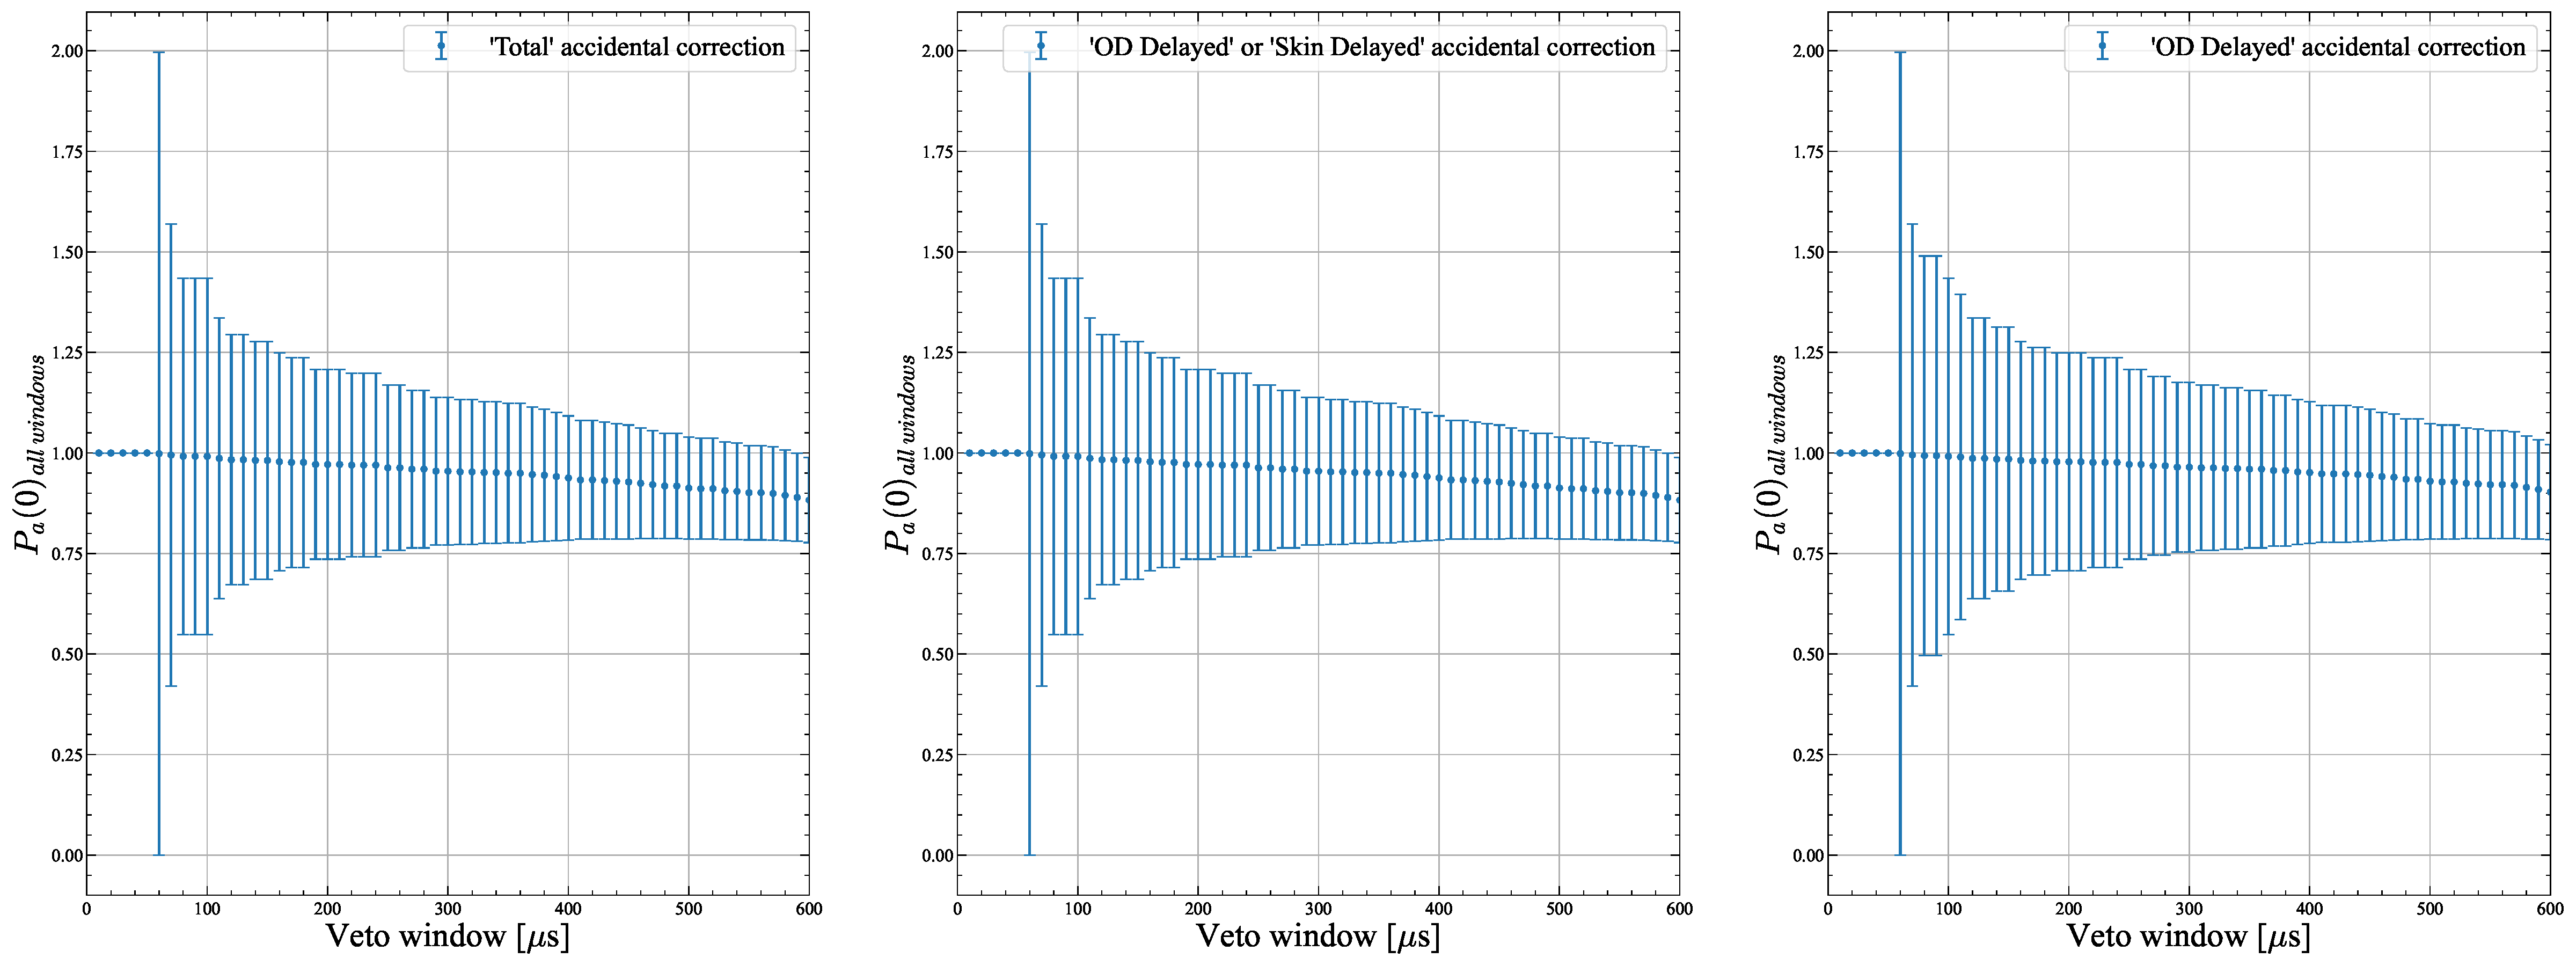
\includegraphics[width=\textwidth]{figures/VetoEfficiency/DDAccCorrectionImpact_P0.pdf}
    \caption{$P_a(>0)_{all\:window}$ DD Accidental correction factors for varying veto window size for different windows of interest.}
    \label{fig:DDAccCorrectionImpact_P0}
\end{figure}

\begin{figure}
    \centering
    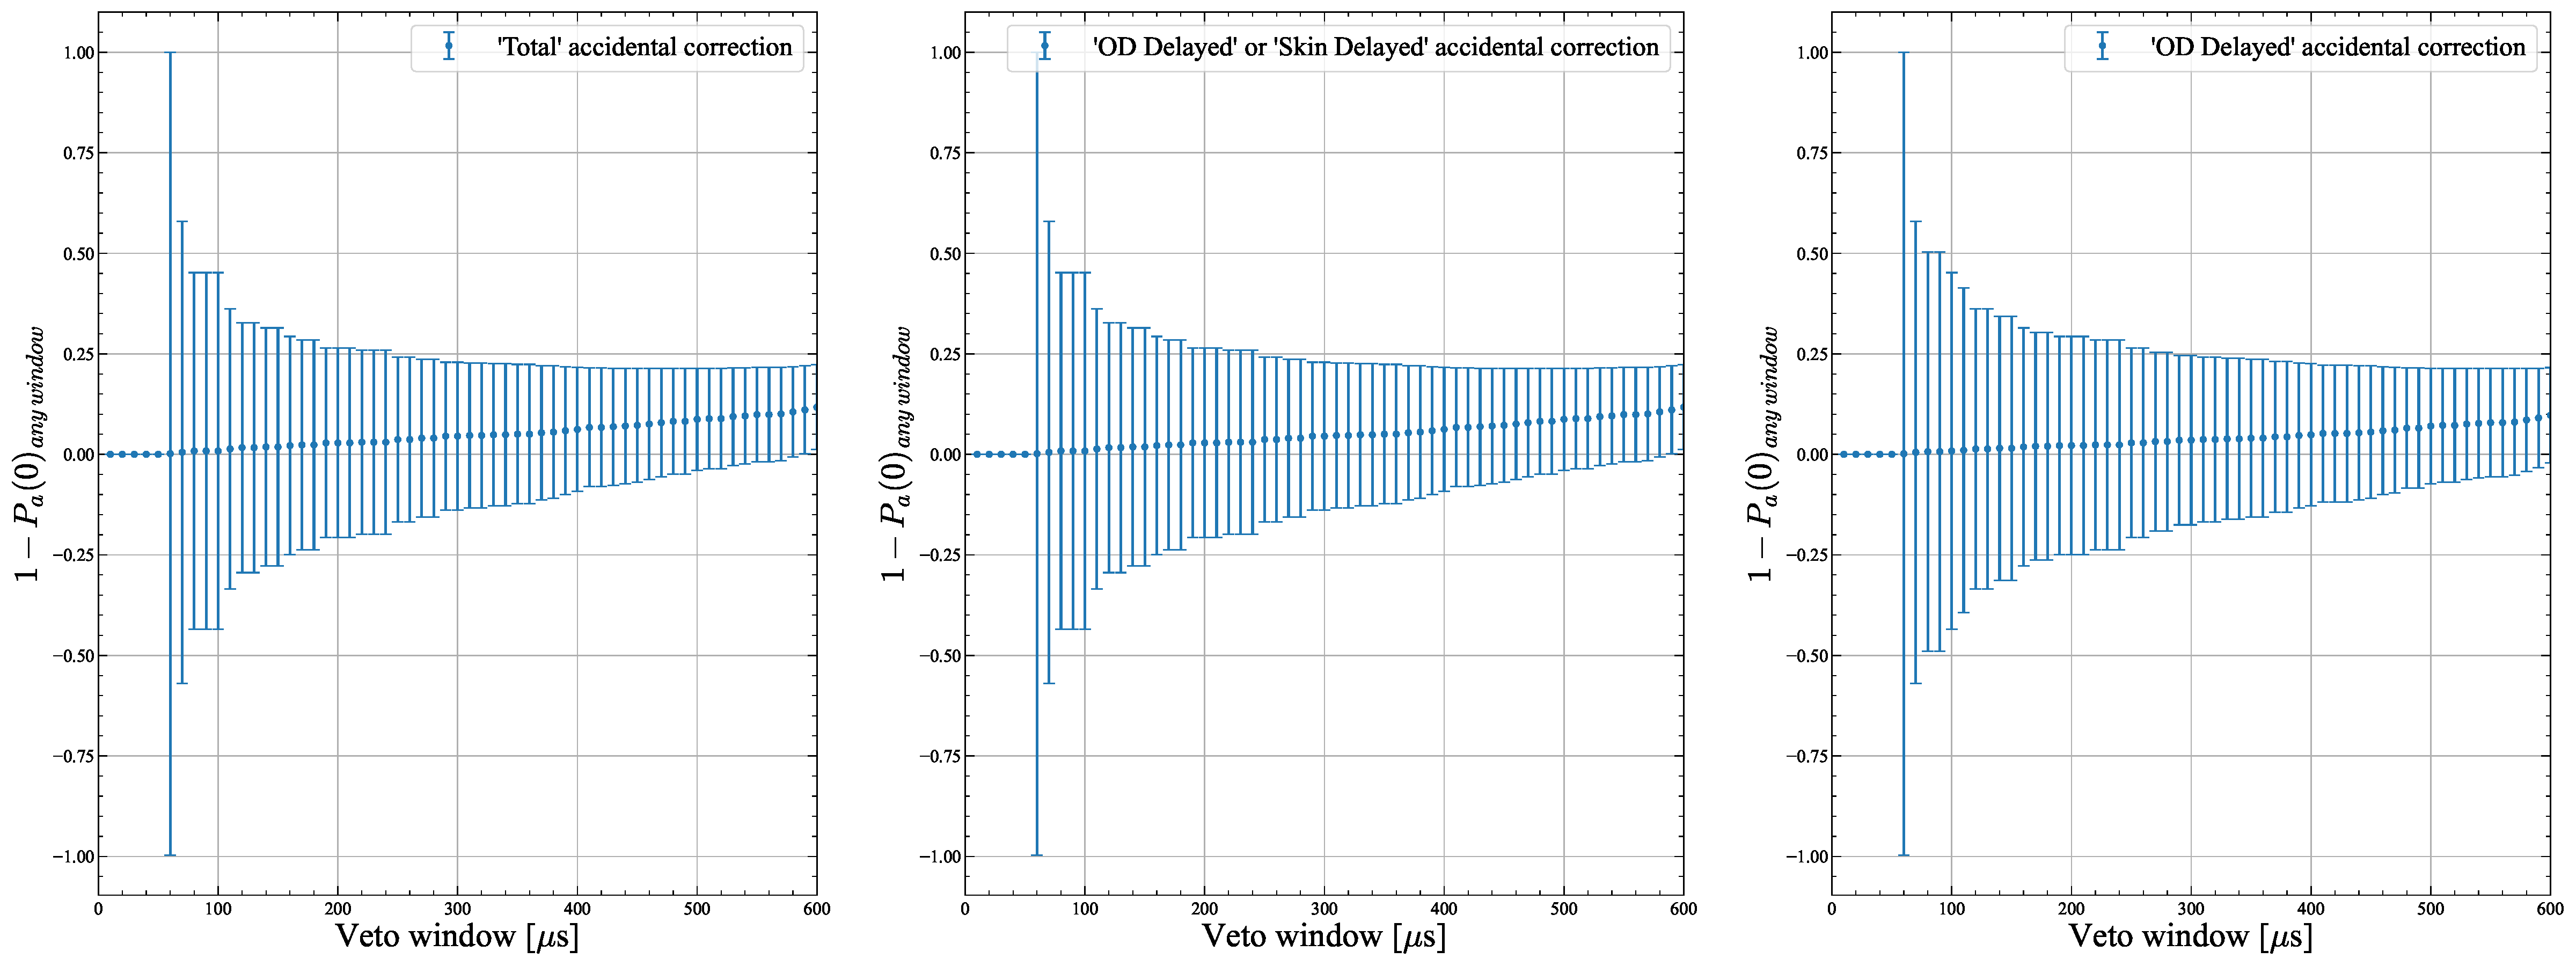
\includegraphics[width=\textwidth]{figures/VetoEfficiency/DDAccCorrectionImpact_1-P0.pdf}
    \caption{$1-P_a(>0)_{any\:window}$DD Accidental correction factors for varying veto window size for different windows of interest.}
    \label{fig:figures/VetoEfficiency/DDAccCorrectionImpact_1-P0}
\end{figure}

\begin{figure}
    \centering
    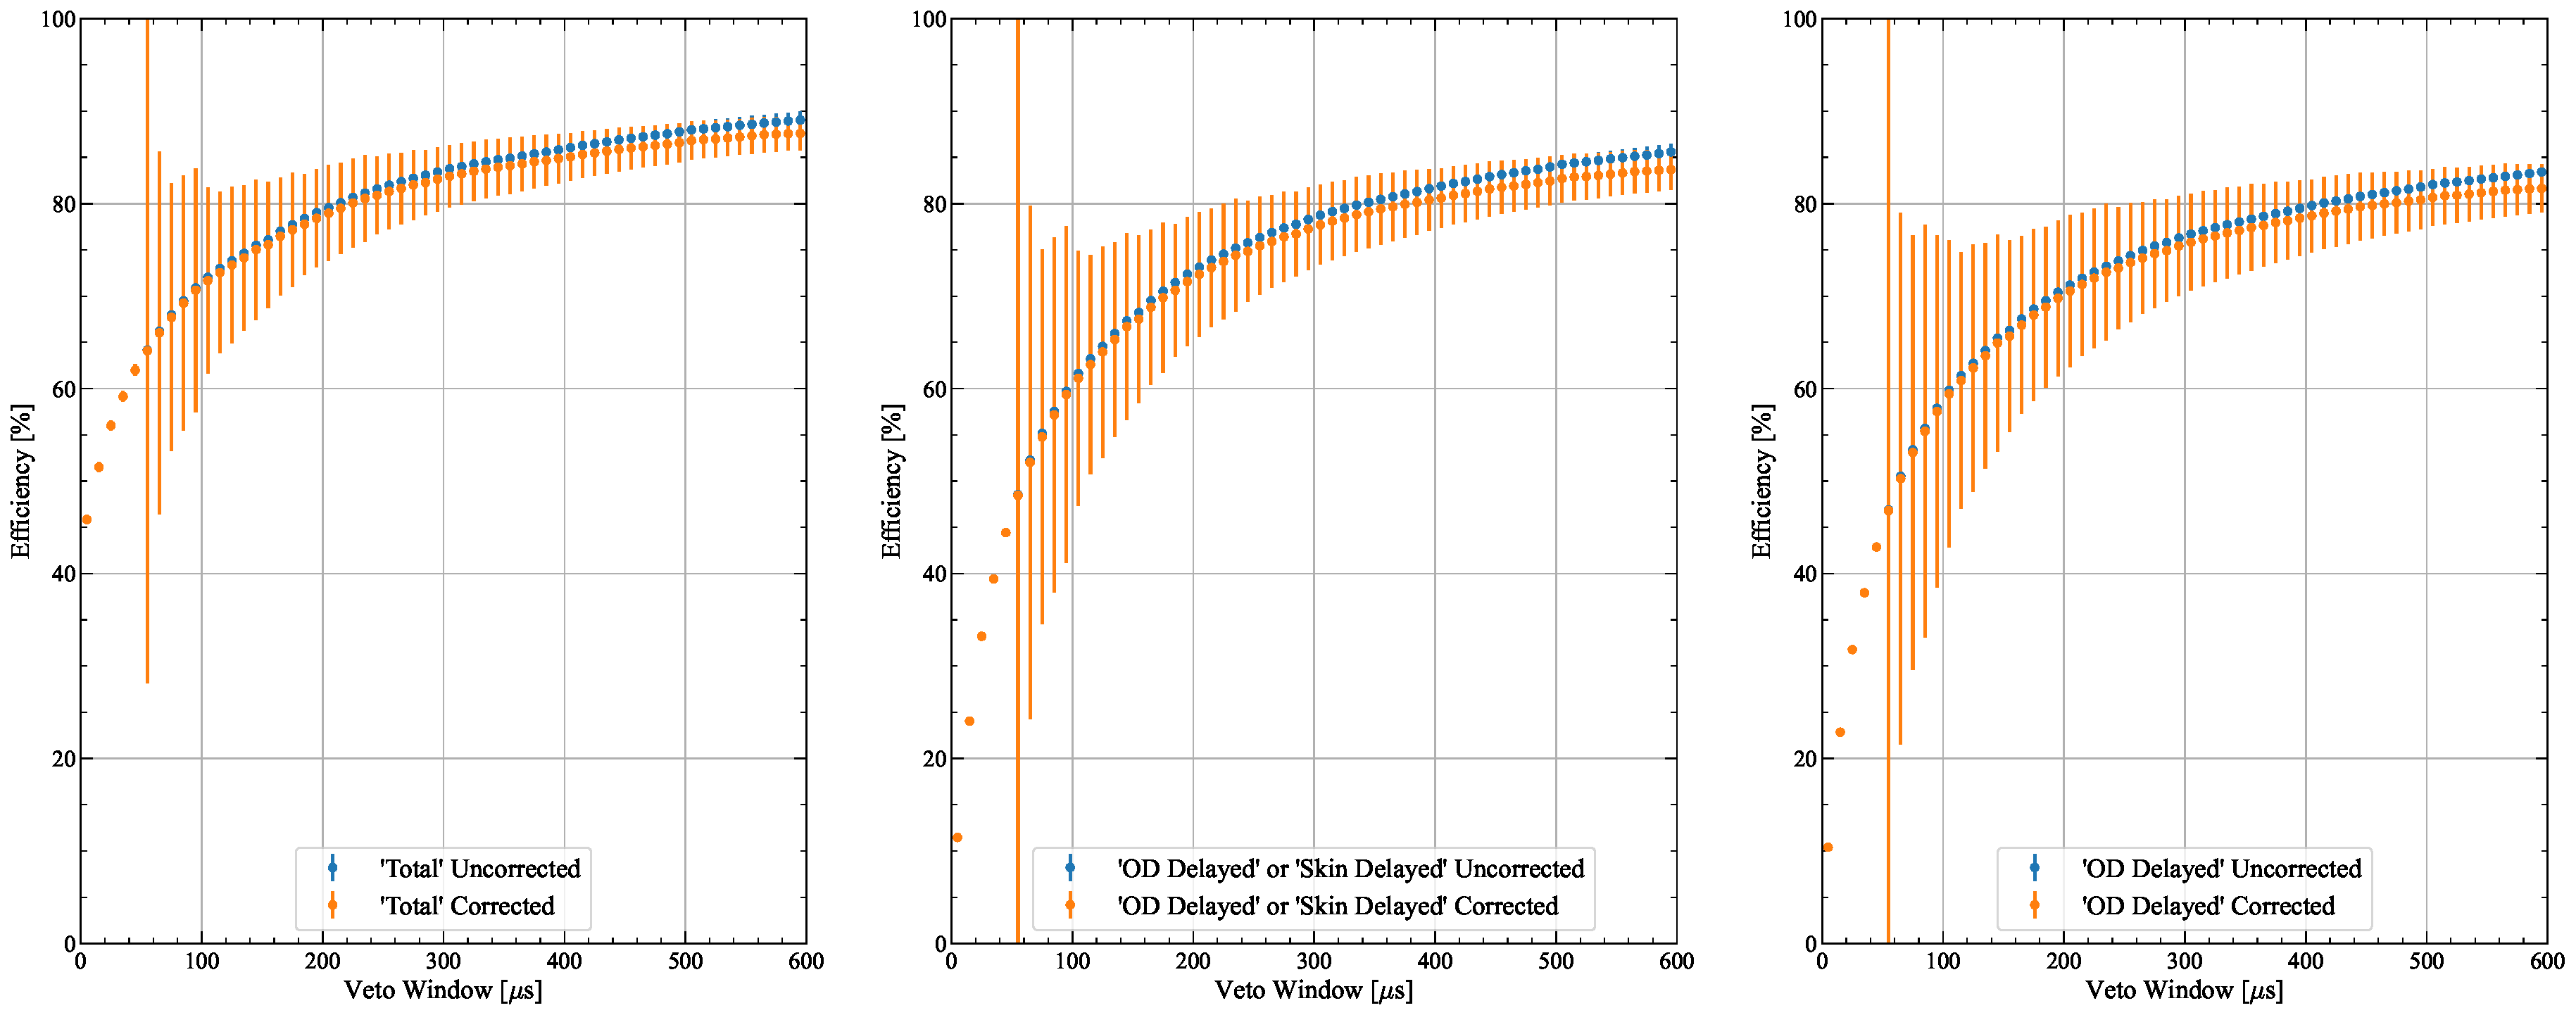
\includegraphics[width=\textwidth]{figures/VetoEfficiency/DDAccCorrectionParameters.pdf}
    \caption{The impact of the accidental correction applied to the different veto efficiencies for the given windows of interest.}
    \label{fig:figures/VetoEfficiency/DDAccCorrectionParameters}
\end{figure}



\subsection{Simulated Neutrons From Calibration Source}
AmLi and DD were simulated using \lstinline{BACCARAT-6.3.5} and \lstinline{LZLAMA-3.5.3}.
On each set of simulation, the cuts listed in \autoref{tab:calibration_simulation_efficiency_cuts} were used.
\begin{table}
    \centering
    \begin{tabular}{c}
     Physics cuts  \\
     \hline
     Single scatter \\
     S1 and S2 threshold \\
     Fiducial Volume \\
     CSD Selection (AmLi Only)\\
    \end{tabular}
    \caption{ALPACA-Core SR3 cuts used on AmLi and DD simulations for determining the efficiency. Each cut is from SR3-cuts-v3.}
    \label{tab:calibration_simulation_efficiency_cuts}
\end{table}
No accidental correction was applied to the simulation data as there are no accidental gammas or neutrons present in the simulation.
How these compare to the data measurements are shown in \autoref{fig:AmLiIneffPlots}-\ref{fig:DDIneffPlots}.
More detailed plots on how the calibration simulations compare to calibration data is in \autoref{sec:simulation_improvements}.

\begin{figure}
\centering
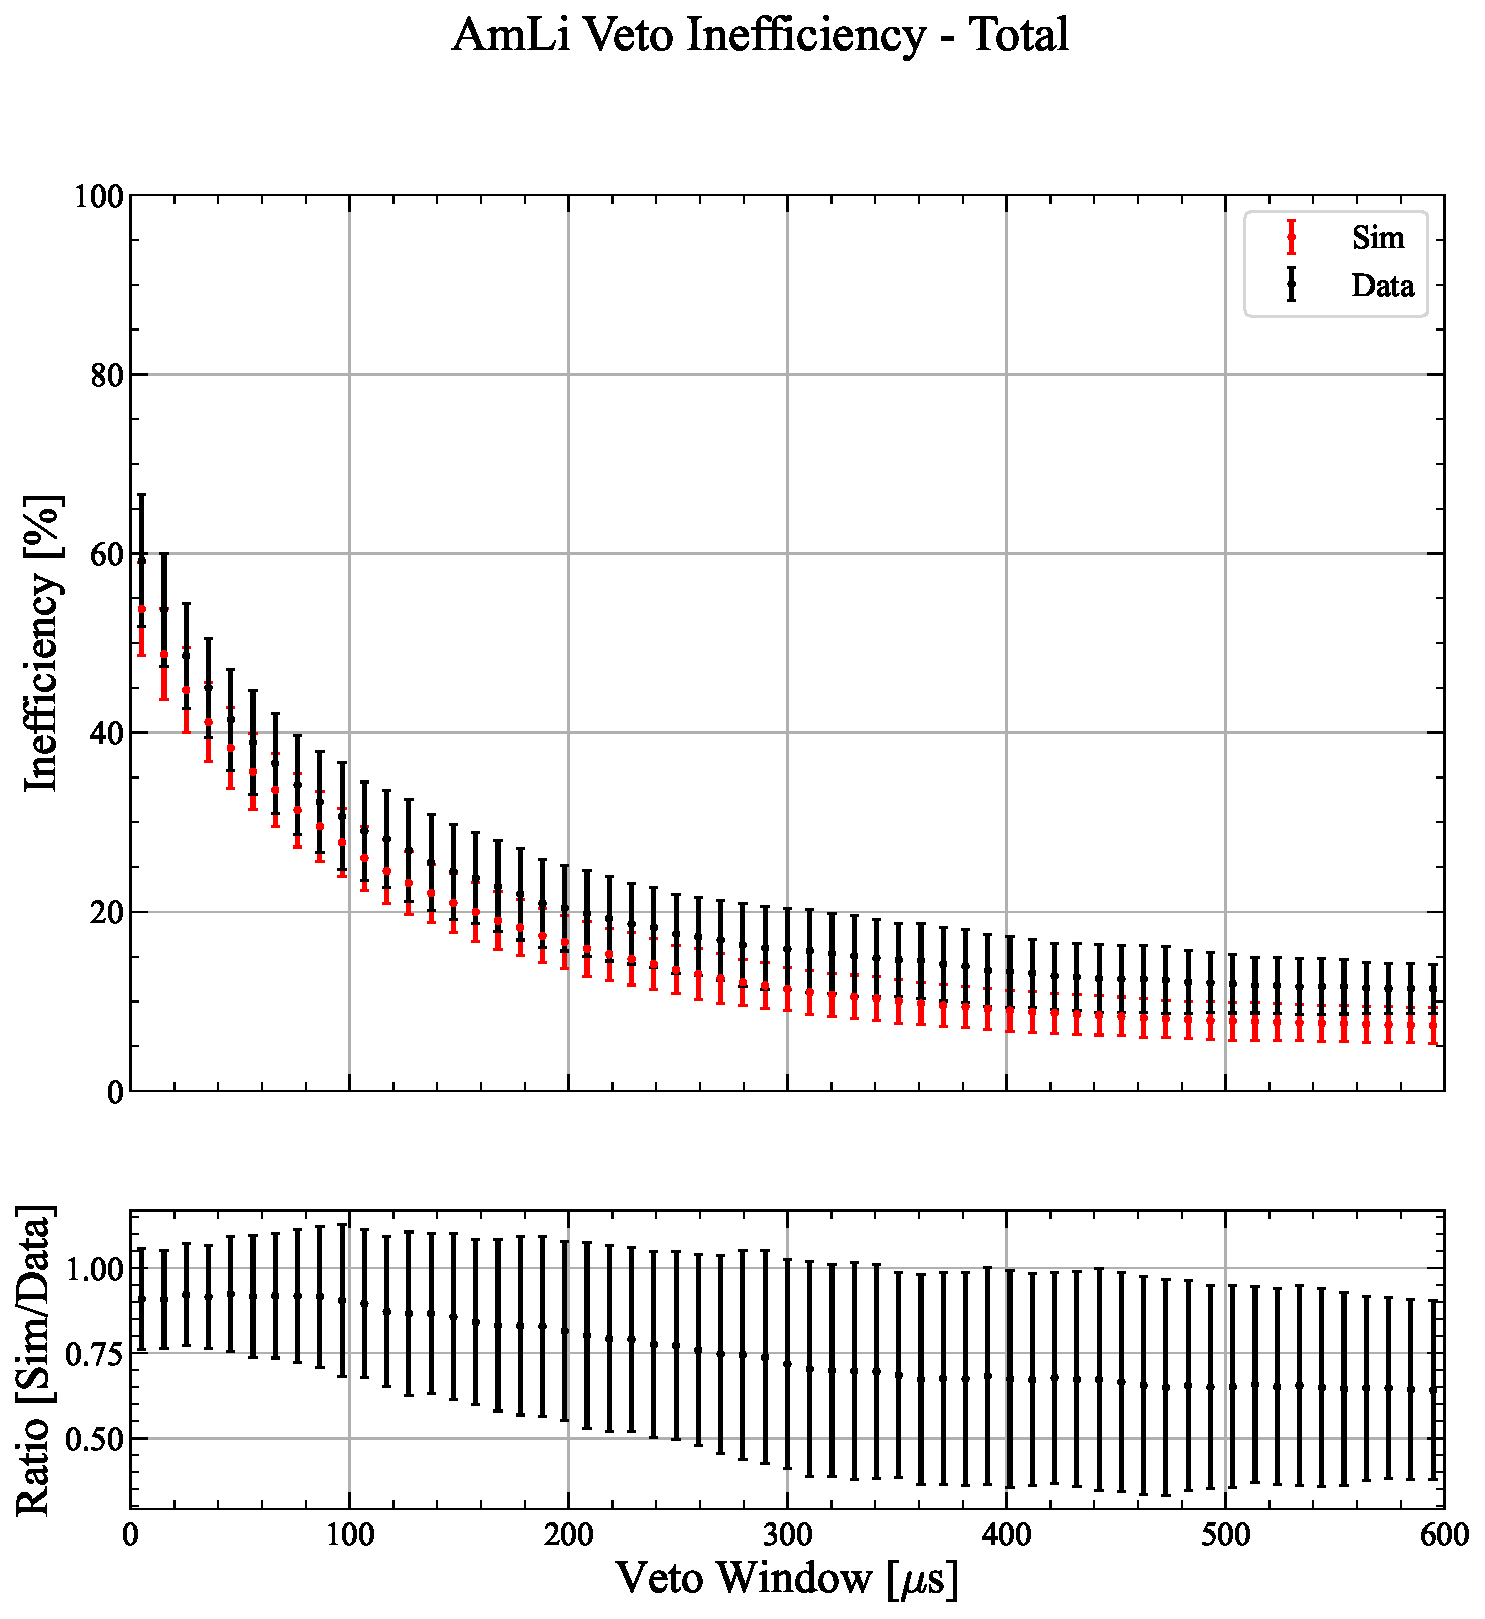
\includegraphics[width=.3\textwidth]{figures/VetoEfficiency/InEff_AmLi_Total_Avg_Ratio.pdf}\hfill
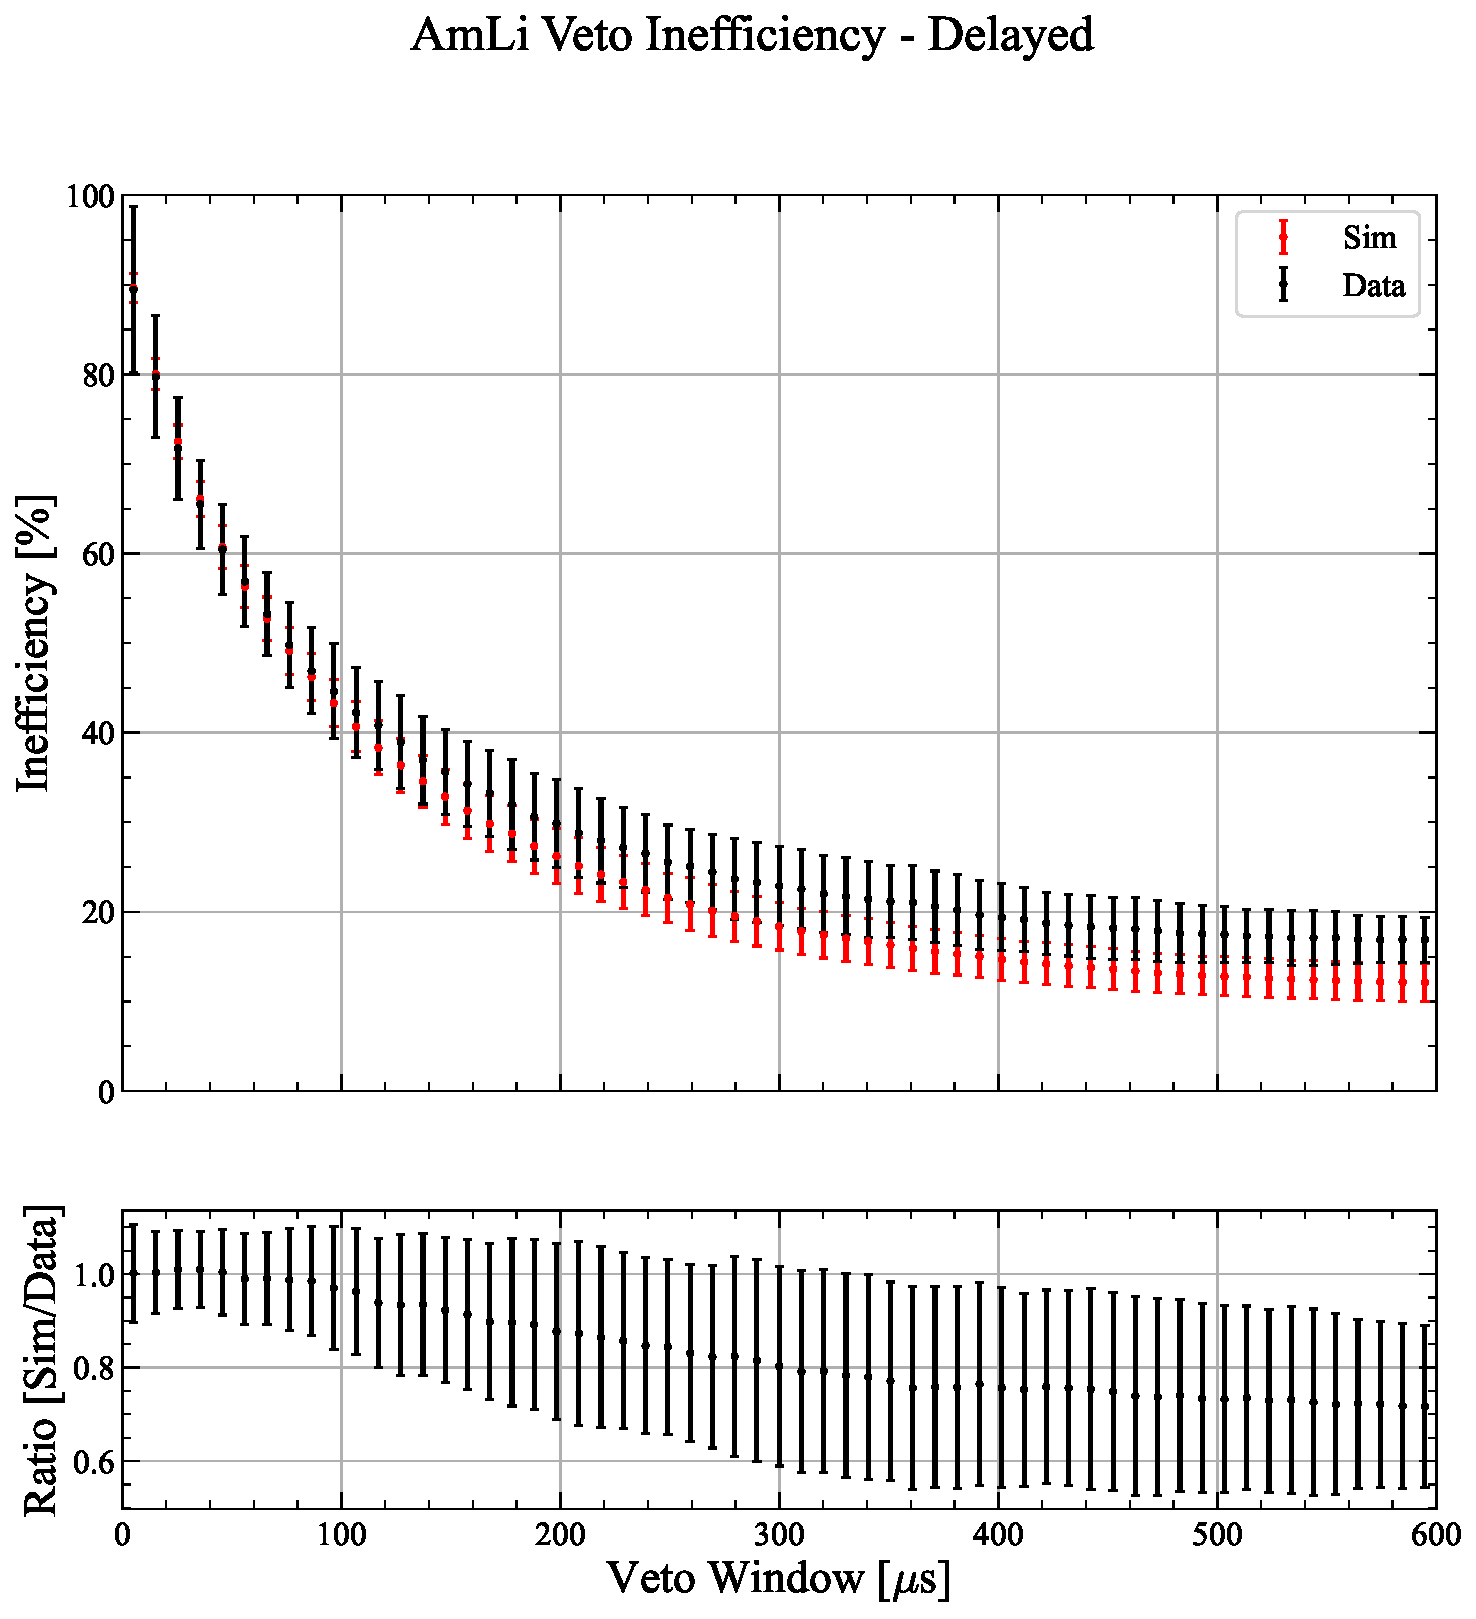
\includegraphics[width=.3\textwidth]{figures/VetoEfficiency/InEff_AmLi_Delayed_Avg_Ratio.pdf}\hfill
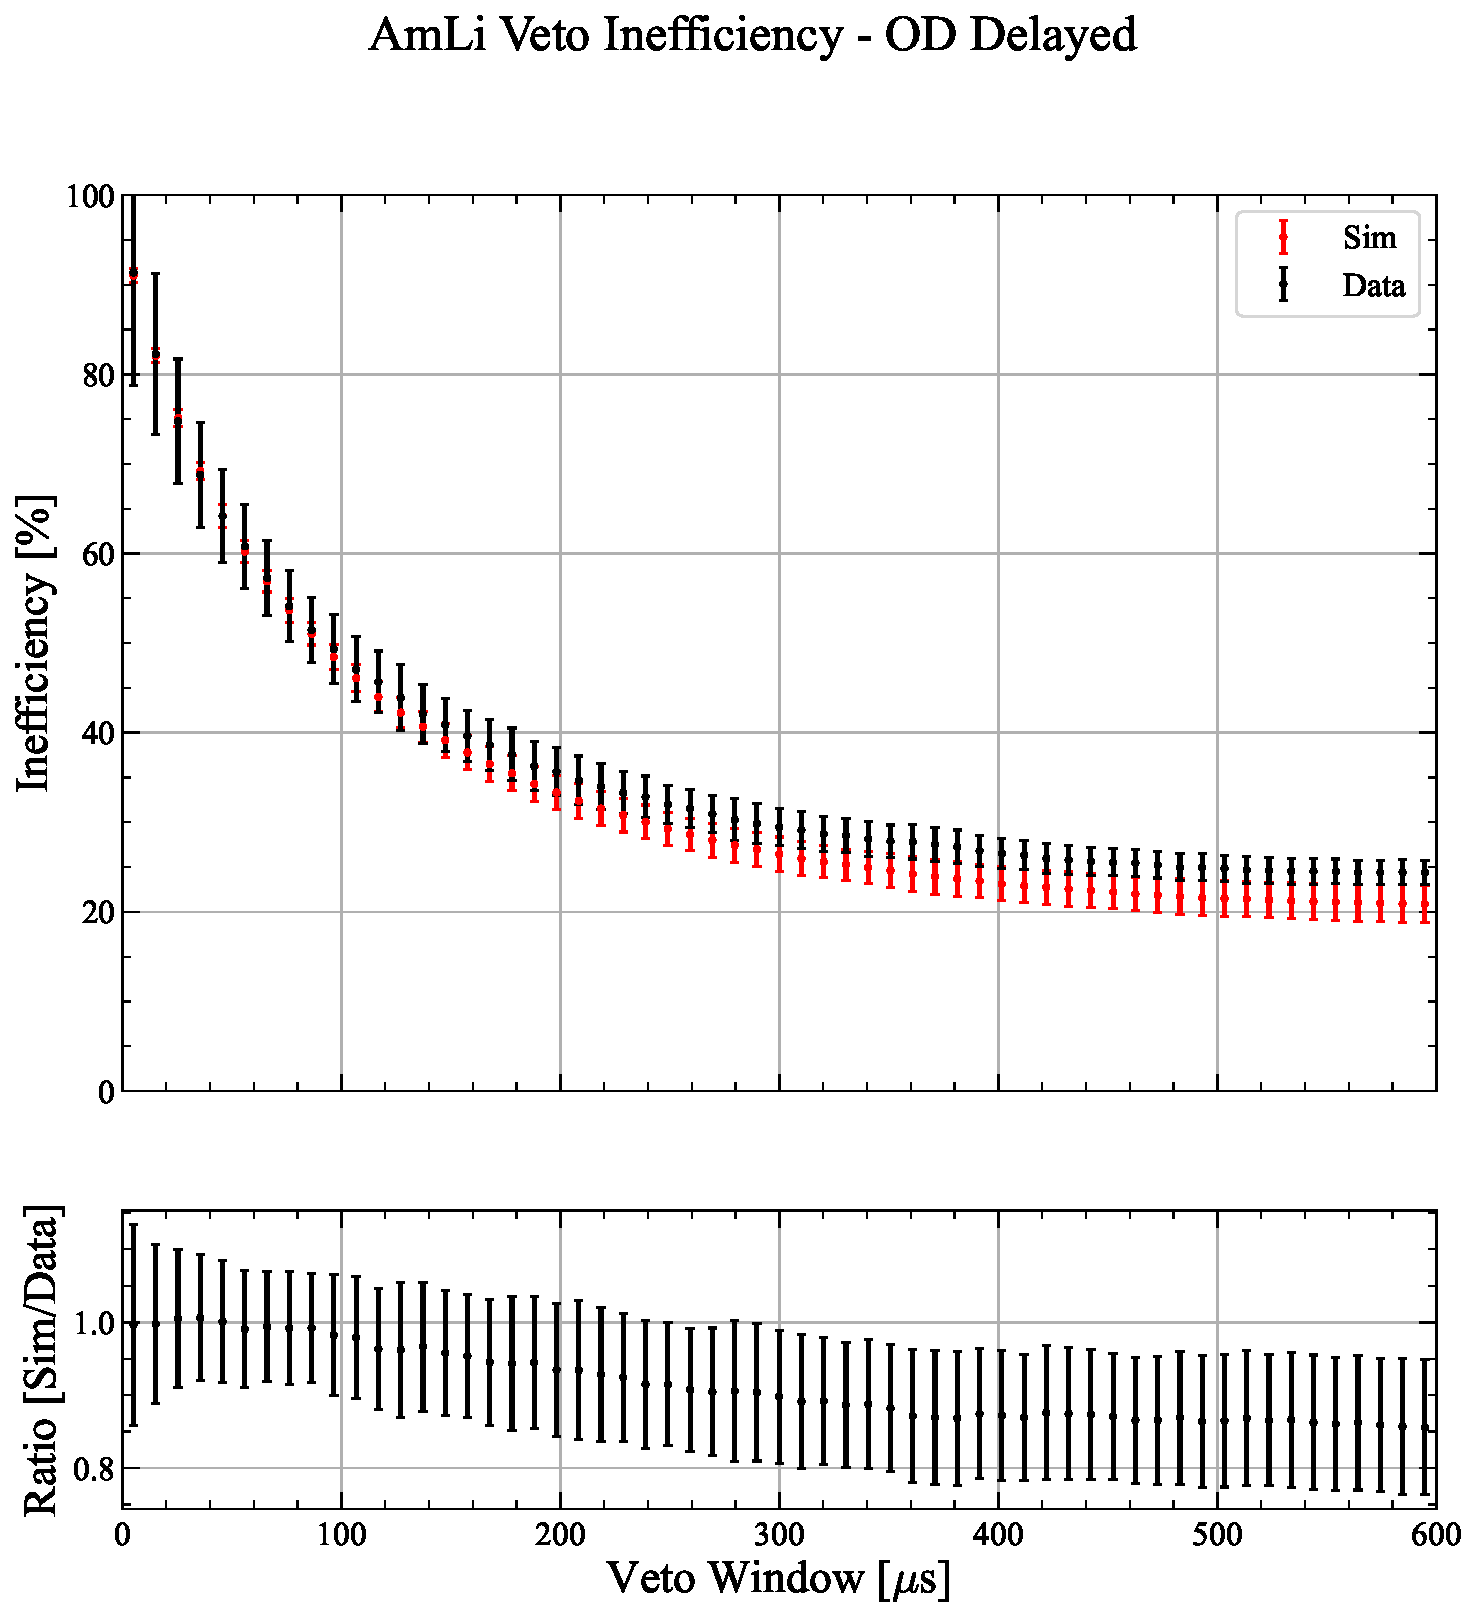
\includegraphics[width=.3\textwidth]{figures/VetoEfficiency/InEff_AmLi_ODDelayed_Avg_Ratio.pdf}
\caption{Inefficiency plots for AmLi, comparing simulations to data.
Left: Total. Middle: Delayed Only. Right: OD Delayed.\\
In each case, the average from all CSD positions are used.}
\label{fig:AmLiIneffPlots}
\end{figure}

\begin{figure}
\centering
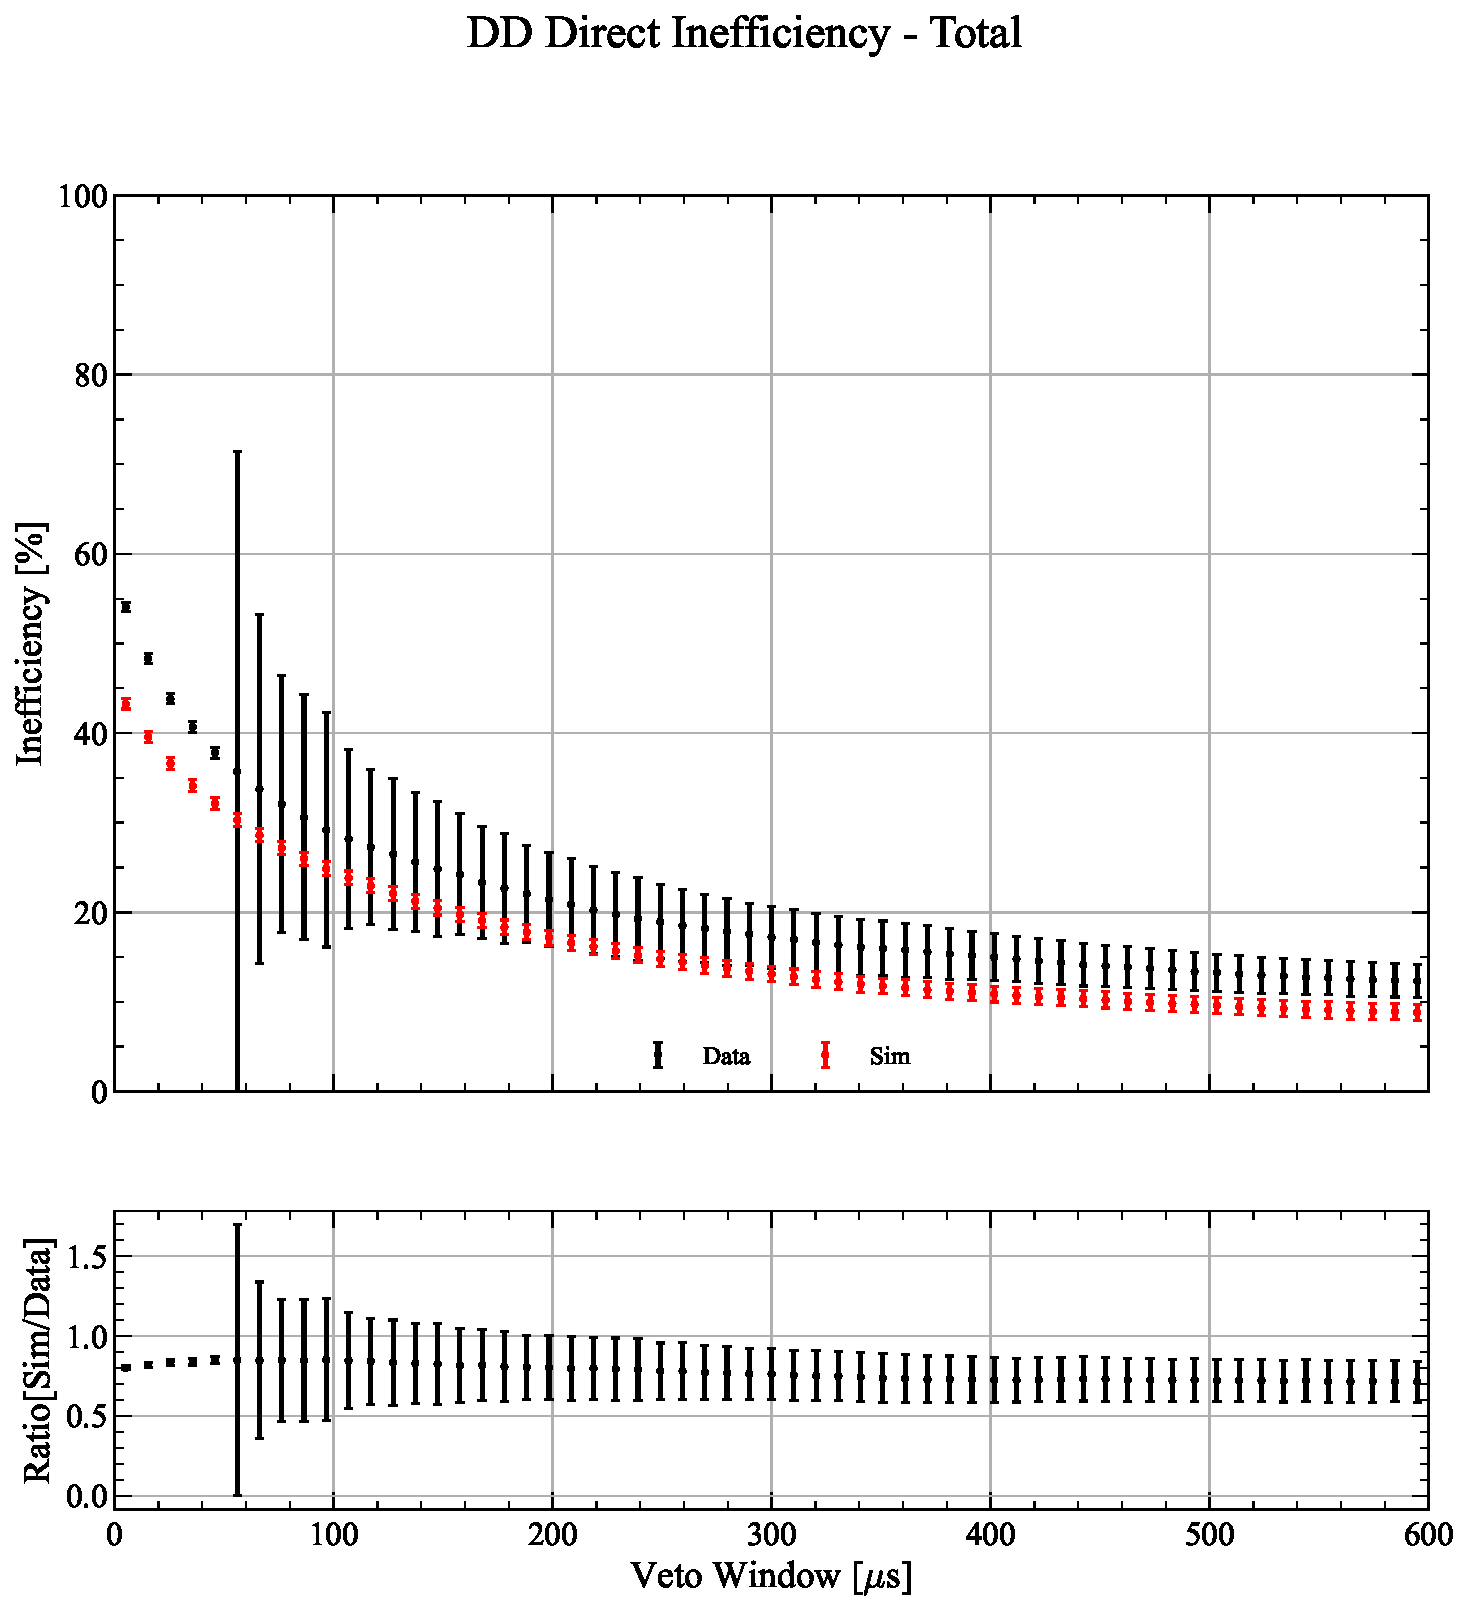
\includegraphics[width=.3\textwidth]{figures/VetoEfficiency/InEff_DDDirect_Total_Ratio.pdf}\hfill
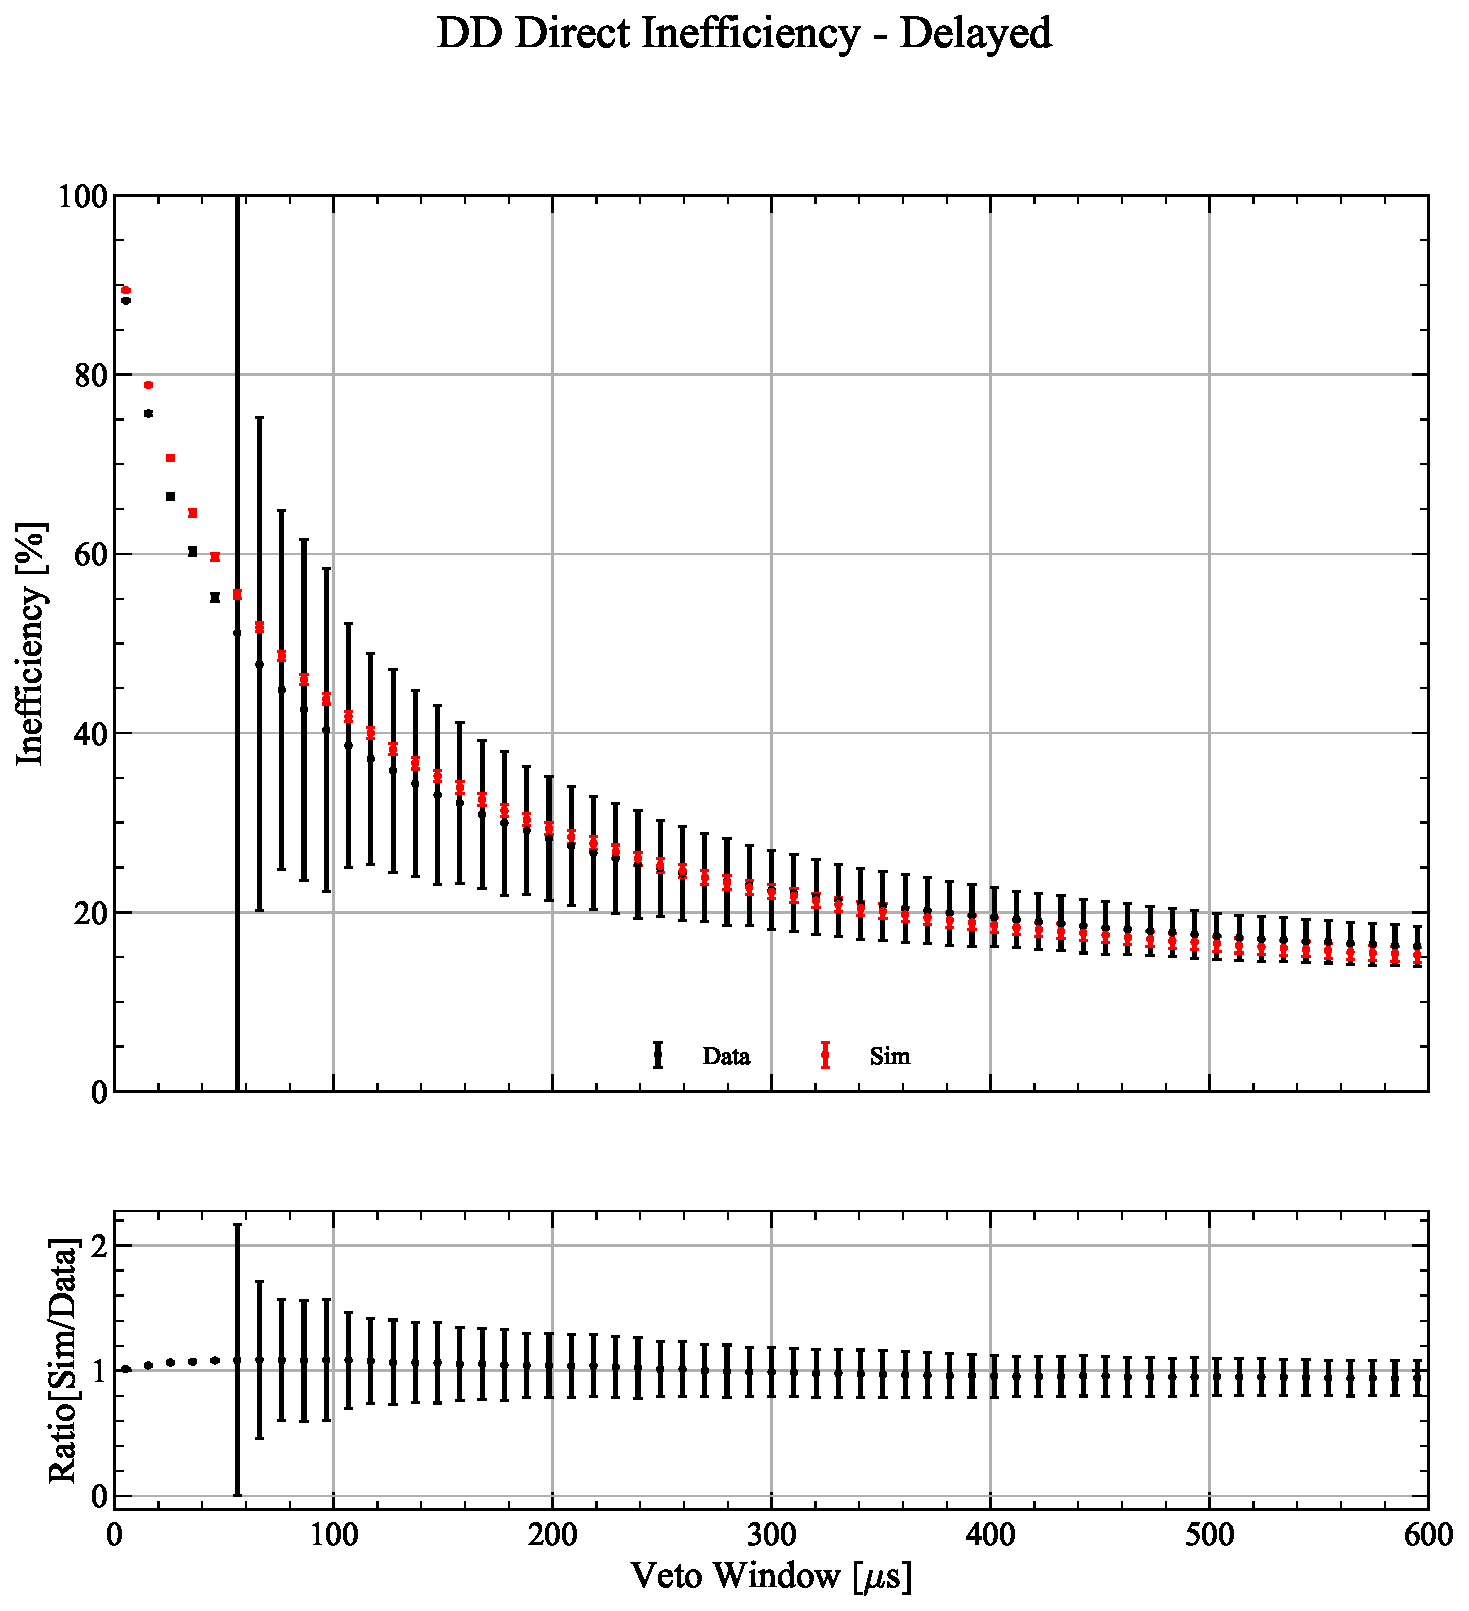
\includegraphics[width=.3\textwidth]{figures/VetoEfficiency/InEff_DDDirect_Delayed_Ratio.pdf}\hfill
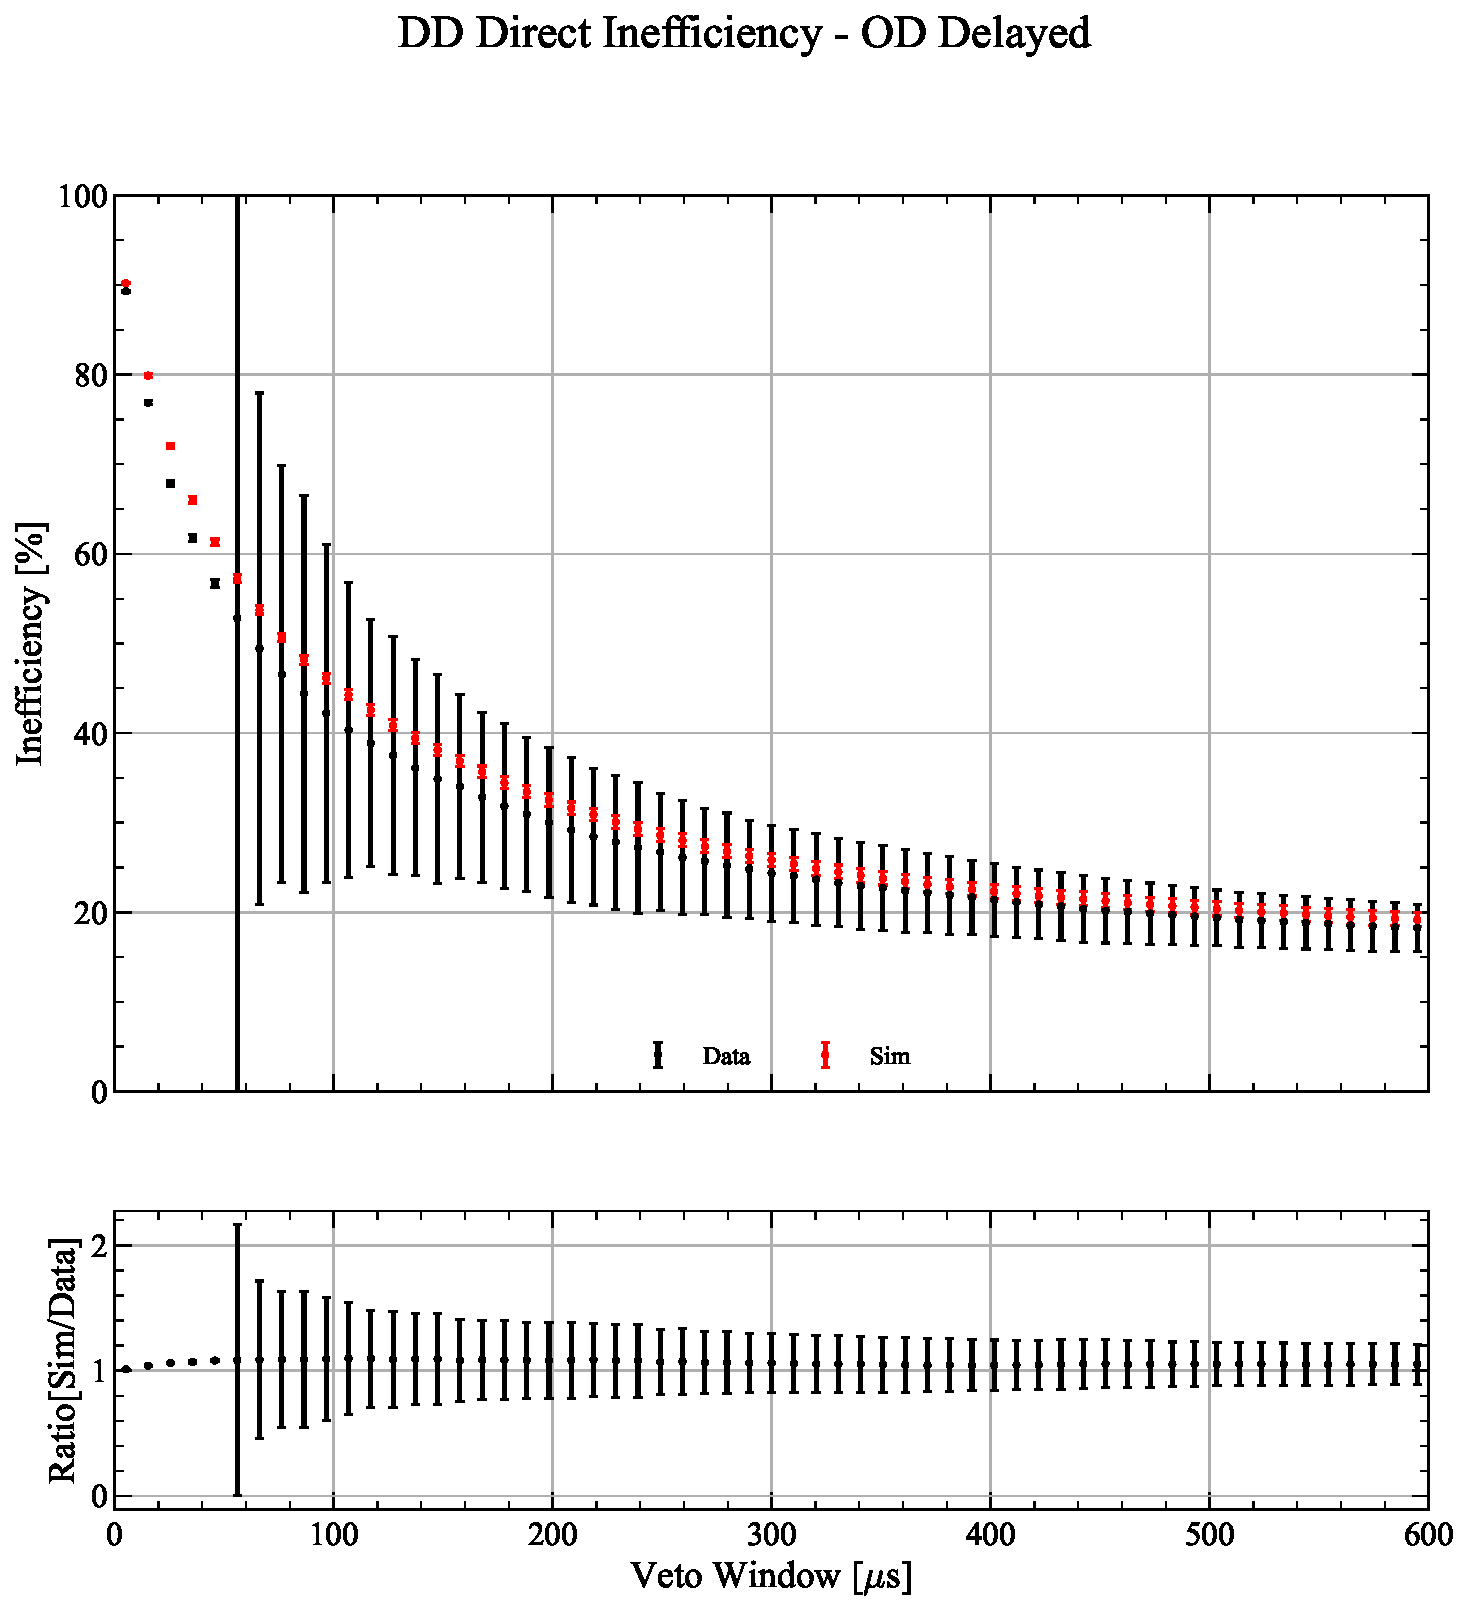
\includegraphics[width=.3\textwidth]{figures/VetoEfficiency/InEff_DDDirect_ODDelayed_Ratio.pdf}
\caption{\centering Inefficiency plots for DD, comparing simulations to data.\\ Left: Total. Middle: Delayed Only. Right: OD Delayed.}
\label{fig:DDIneffPlots}
\end{figure}

\subsection{Background Neutrons}
The detector-NR simulations were simulated as part of the official production of SR3-BG. Each of the 644 components were simulated using BACCARAT-6.3.5 and LZLAMA-3.5.3.
On these events, the cuts listed in \autoref{tab:detector_nr_simulation_efficiency_cuts} were applied.
The efficiency of tagging neutrons from USF and ($\alpha$,n) events are shown in \autoref{fig:detector_nr_efficiency}.
Also shown is the total efficiency.

\begin{table}
    \centering
    \begin{tabular}{c}
     Physics cuts  \\
     \hline
     Single scatter \\
     S1 and S2 threshold \\
     Fiducial Volume 
    \end{tabular}
    \caption{ALPACA-Core SR3 cuts used on Detector-NR simulations for determining the efficiency. Each cut is from SR3-cuts-v3.
    }
    \label{tab:detector_nr_simulation_efficiency_cuts}
\end{table}


\begin{figure}
    \centering
    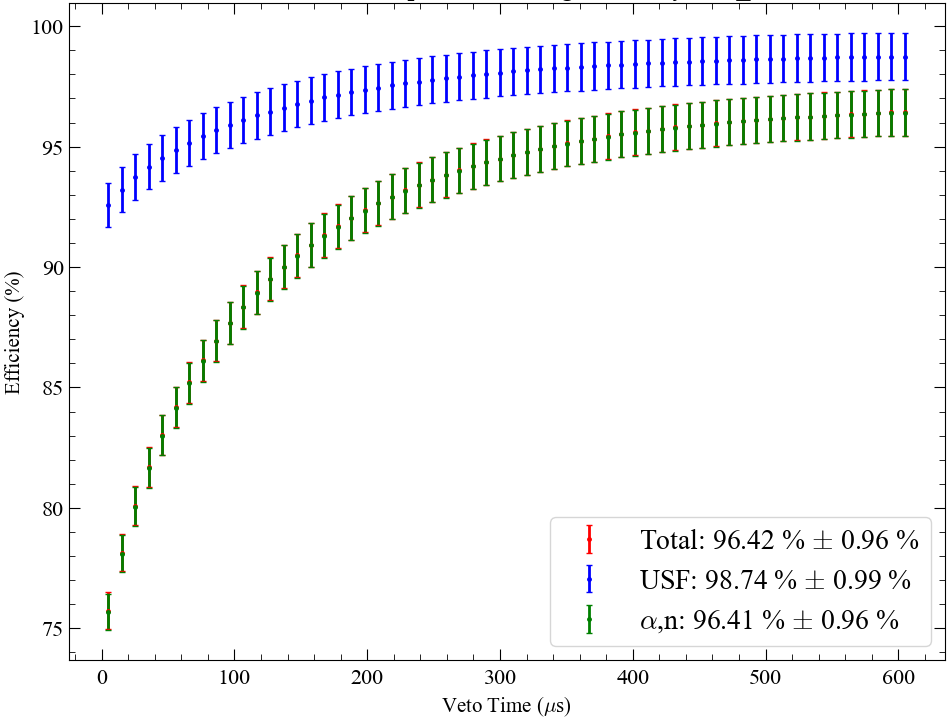
\includegraphics[width=0.5\textwidth]{figures/VetoEfficiency/det_nr_efficiency.png}
    \caption{Efficiency for tagging a neutron on Detector-NR simulations.}
    \label{fig:detector_nr_efficiency}
\end{figure}

\clearpage
\subsection{Background Neutron Efficiency From Data}
Shown in \autoref{fig:efficiency_summary} is the neutron veto efficiency from each calibration source from data and simulation.
Also shown is the efficiency from simulated background neutrons.
The Z-position of each point is calculated from the \lstinline{mean(driftTime)} of events which pass the selection.
For the Detector-NR, the events were split up into Z-sections by the following;
\begin{lstlisting}
    def SR3ZThirds_Cut(driftTime_us: float, position='top'):
        if position == 'top':
            return ((driftTime_us < 350.) & (driftTime_us > 71.))
        elif position == 'mid':
            return ((driftTime_us < 700.) & (driftTime_us > 350.))
        elif position == 'bot':
            return ((driftTime_us < 1030.) & (driftTime_us > 700.))
\end{lstlisting}
This \lstinline{driftTime} splitting was performed so that comparing to calibration points was easier, but in evaluating the total efficiency, it is not used.

Shown in \autoref{tab:final_veto_efficiency} are the veto efficiencies of all calibration sources for both simulations and data.
The value we care about is the background neutron efficiency, $\epsilon_{\textrm{bg data}}$, or inefficiency, $\zeta_{\textrm{bg data}}$.
There are a number of ways in which this can be calculated, which are described below.
The proposed option is no.2, of 7.8$\pm$4.3\%; or quote as 8$\pm$4.
\autoref{tab:efficiency_options} contains the results of each approach.

\paragraph{Option 1}:
We take the average simulation calibration efficiency, so the mean of AmLi (92.8\%) and DD (91.8\%), then we have 92.3\%.
We take the average data calibration efficiency, 88.6\% for AmLi and 87.7\%, for DD we have 88.2\%.
The ratio, $\Delta$, of the simulation calibrations and the data calibration can then be used as a scaling factor on the simulation background.
This process is expressed in \autoref{eq:efficiency_option1}, and gives an efficiency of 92.1\%.
In this case, the uncertainty is 4.5\%, made up from a statistical error from the simulations (0.96\%), and 4.3 from the scaling.

\begin{align}
    \epsilon_{\textrm{cal. data}} &= \frac{\epsilon_{\textrm{data DD}} + \epsilon_{\textrm{data AmLi}}}{2} \\
    \epsilon_{\textrm{cal. sims}} &= \frac{\epsilon_{\textrm{sims DD}} + \epsilon_{\textrm{sims AmLi}}}{2} \\
    \Delta &= \frac{\epsilon_{\textrm{cal. data}}}{\epsilon_{\textrm{cal. sims}}} \\
    \epsilon_{\textrm{bg data}} &= \Delta \times \epsilon_{\textrm{bg sims}}
    \label{eq:efficiency_option1}
\end{align}

\paragraph{Option 2}:
We take the average simulation calibration efficiency, so the mean of AmLi (92.8\%) and DD (91.8\%), then we have 92.3\%.
We take the average data calibration efficiency, 88.6\% for AmLi and 87.7\%, for DD we have 88.2\%.
The difference, $\Lambda$, between the simulation calibrations and the data calibrations can then be used as a systematic uncertainty on the simulation backgrounds.
This process is expressed in \autoref{eq:efficiency_option2}, and gives an efficiency of 92.2\%.
In this case, the uncertainty is 4.3\%, made up from a statistical error from the simulations (0.96\%), and 4.22 from the subtraction.

\begin{align}
    \epsilon_{\textrm{cal. data}} &= \frac{\epsilon_{\textrm{data DD}} + \epsilon_{\textrm{data AmLi}}}{2} \\
    \epsilon_{\textrm{cal. sims}} &= \frac{\epsilon_{\textrm{sims DD}} + \epsilon_{\textrm{sims AmLi}}}{2} \\
    \Lambda &= \epsilon_{\textrm{cal. sims}} - \epsilon_{\textrm{cal. data}} \\
    \epsilon_{\textrm{bg data}} &= \epsilon_{\textrm{bg sims}} - \Lambda
    \label{eq:efficiency_option2} 
\end{align}

\paragraph{Option 3}:
We take the average simulation calibration inefficiency, so the mean of AmLi ($100 - 92.8 = 7.2$\%) and DD ($100 - 91.8 = 8.3$\%), then we have 7.7\%.
We take the average data calibration inefficiency, 11.5\% for AmLi and 12.3\% for DD, we have 11.9\%.
The ratio, $\Delta$, of the simulation calibrations and the data calibration can then be used as a scaling factor on the simulation background.
This process is expressed in \autoref{eq:efficiency_option3}, and gives an inefficiency of 5.5.
In this case, the uncertainty is 2.8\%, made up from a statistical error from the simulations (0.96\%), and 1.8 from the subtraction.

\begin{align}
    \zeta_{\textrm{cal. data}} &= 100 - \frac{\epsilon_{\textrm{data DD}} +\epsilon_{\textrm{data AmLi}}}{2} \\
    \zeta_{\textrm{cal. sims}} &= 100 - \frac{\epsilon_{\textrm{sims DD}} + \epsilon_{\textrm{sims AmLi}}}{2} \\
    \Delta &= \frac{\zeta_{\textrm{cal. data}}}{\zeta_{\textrm{cal. sims}}} \\
    \zeta_{\textrm{bg data}} &= \zeta_{\textrm{bg sims}} \times \Delta 
    \label{eq:efficiency_option3} 
\end{align}


\clearpage
\begin{table}
\begin{tabular}{l|l|l}
Source         & Simluation     & Data           \\ \hline
AmLi (average) & 92.8$\pm$2.0\% & 88.6$\pm$2.7\% \\
DD (Direct)    & 91.8$\pm$1.0\% & 87.7$\pm$1.8\% \\
Detector-NR    & 96.4$\pm$1.0\% & 92.2$\pm$4.3 
\end{tabular}
    \caption{Summary of veto efficiencies.
    The Detector-NR Data value assumes that option 2 is used.}
    \label{tab:final_veto_efficiency}
\end{table}

\begin{table}
\begin{tabular}{l|l|l}
Option & efficiency & inefficiency \\ \hline
No. 1  & 92.1$\pm$4.5 & 7.9$\pm$4.5\\
No. 2  & 92.2$\pm$4.3 & 7.8$\pm$4.3\\
No. 3  & 94.5$\pm$2.8 & 5.5$\pm$2.8
\end{tabular}
    \caption{Summary of veto efficiencies and inefficiencies as determined from each approach.}
    \label{tab:efficiency_options}
\end{table}

\begin{figure}
    \centering
    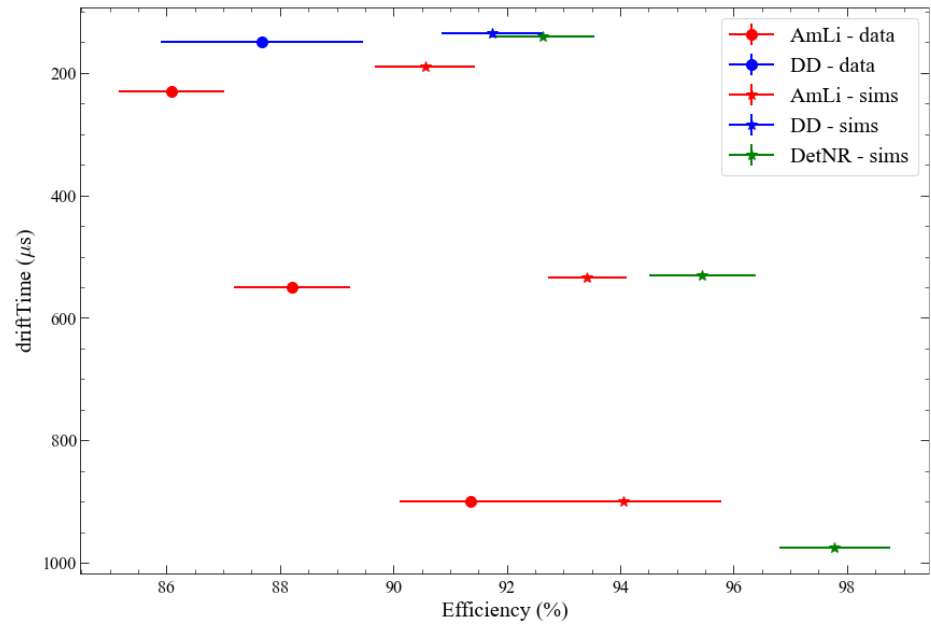
\includegraphics[width=0.8\textwidth]{figures/VetoEfficiency/efficiency_summary.png}
    \caption{Summary of efficiency from all simulations and calibration sources.
    The CSD sources are averaged at each height.
    Circle marks are from data.
    Start marks are from simulations.
    The \lstinline{driftTime} is defined as when \lstinline{mean(driftTime)} of events which pass all other cuts.
    }
    \label{fig:efficiency_summary}
\end{figure}

\section{Veto Efficiency and the WIMP search}